\documentclass[12pt]{article}
\usepackage[margin=1in]{geometry}
\usepackage{amsmath,amssymb}
\usepackage{graphicx}
\usepackage{booktabs,array}
\usepackage{setspace}
\usepackage[colorlinks=true,
            urlcolor=blue,
            linkcolor=black,
            citecolor=black]{hyperref}
\usepackage{float}
\usepackage{threeparttable}
\usepackage{tikz}
\usepackage{pgfplots}
\usepackage[utf8]{inputenc}
\usepackage{tabularx}
\usepackage{calc} % for calculating minipage widths
\usepackage{algorithm}
\usepackage{algpseudocode}
\usepackage{amsmath,amssymb,amsfonts}
\usepackage[final]{microtype}
\usepackage{setspace}
\usepackage[backend=biber, style=apa]{biblatex}
\usepackage{booktabs}
\usepackage{multirow}
\usepackage{threeparttable}
\usepackage{makecell}
\usepackage{array}
\usepackage{adjustbox} % or graphicx for resizebox

\pgfplotsset{compat=1.17}
\addbibresource{references.bib}  % Gunakan file bib yang disediakan
\onehalfspacing
\DeclareSourcemap{
  \maps[datatype=bibtex]{
    \map{
      \step[fieldsource=doi, final]
      \step[fieldset=url, null]
      \step[fieldset=eprint, null]
    }
  }
}

\newcommand{\keywords}[1]{
  \vspace{3pt}
  \noindent\textbf{\textit{Keywords}:} #1
  \vspace{3pt}
}


% Document Metadata
\title{Aggregate retail sales forecasting with SKU-level set representation learning }

\author{%
    \begin{tabular}{c}
        Shaohui Ma, Shengkai Wang\\
        \href{mailto:shaohui.ma@nau.edu.cn}{\underline{shaohui.ma@nau.edu.cn}} \\
        School of Business, Nanjing Audit University \\
        No.86 Yushan West Road, Nanjing, China,211815 \\
    \end{tabular}%
}
\date{April, 2026}

\begin{document}

\pagenumbering{gobble}
\maketitle
\newpage

\begin{abstract}
  Retail forecasting often involves a mismatch between the granularity of prediction targets and that of informative explanatory variables. In many practical settings, forecasts are required at aggregate levels such as the total sales at the store--department or the total sales at the store--category, whereas key demand drivers, including prices, promotions, and product-specific demand dynamics, are observed at the SKU level. Directly aggregating such fine-grained information may therefore lead to substantial information loss. This study formulates aggregate retail forecasting as a cross-level representation learning problem and proposes a set-based forecasting framework that integretes SKU level information to improve aggregate sales prediction. The framework first encodes SKU-level future trajectories into latent temporal representations and then aggregates the resulting SKU embeddings into an aggregate-level forecasting representation through learned set-based modules. Three variants are considered, based on gated pooling, Deep Sets, and Set Transformer aggregation, respectively. The framework optimizes forecasting objectives at the aggregate level and supports both point forecasting and probabilistic forecasting. Empirical evaluation on multiple aggregate forecasting tasks shows that the proposed cross-level models consistently outperform direct aggregate-level baselines, bottom-up approaches, and handcrafted child-summary benchmarks. The Set Transformer variant delivers the strongest overall performance, while the Gated Pooling variant performs very closely and achieves the best results on several individual tasks. The gains are especially pronounced at more aggregated target levels, where the mismatch between target granularity and information granularity is greater. Robustness checks using rolling-origin evaluation and alternative SKU sample fractions confirm the stability of the findings. Overall, the results demonstrate the value of set-based cross-level representation learning for aggregate retail sales forecasting.

  \vspace{1em}

  \textbf{Keywords}: retail forecasting; aggregate sales forecasting; cross-level prediction; set representation learning

\end{abstract}


\newpage
\clearpage
\pagenumbering{arabic}
\setcounter{page}{1}

\section{Introduction}

Retail demand forecasting is ofen required at multiple levels of aggregation. In practice, retailers need forecasts not only for individual stock keeping units (SKUs), but also for more aggregated units such as store–department, store–category, and regional business units \parencite{fildes2022retail}. These aggregate forecasts play an important role in tactical and strategic retail decisions, including category management, budgeting, promotion planning, and resource allocation \parencite{Fisher2018UsingDataBigData}. Aggregate forecasting in retail is complicated by a persistent mismatch between the level at which forecasts are required and the level at which much of the most informative explanatory information is observed. In many operational settings, the target of interest is an aggregate sales series, whereas key demand drivers—such as prices, promotions, assortment composition, and product-specific demand dynamics—are naturally defined at the SKU level. When such fine-grained information is aggregated prematurely, part of its predictive content may be weakened or distorted.

A common practice in aggregate retail forecasting is to align the modeling level with the target level \parencite{fildes2022retail}. Under this strategy, historical sales and explanatory variables are first aggregated to the target level, and a forecasting model is then trained directly on the resulting aggregate series. This approach is simple and operationally convenient, but it may fail to preserve important heterogeneity across constituent SKUs \parencite{MA2017680}. When these variables are aggregated through summary operations such as averaging or summation, their predictive meaning may be weakened or even distorted. For example, if two SKUs have different price elasticities and follow alternating discount schedules, the average price at the aggregate level may no longer convey the correct economic signal for future sales. Similar distortions may arise for promotion variables, assortment structure, and product mix. As a result, the conventional ``aggregate first, then model'' paradigm may fail to exploit the most informative signals available in retail data.

A common strategy in retail forecasting is therefore to align the modelling level with the target level: explanatory variables are aggregated to the forecast target, and a forecasting model is estimated directly on the resulting aggregate series. This approach is simple and operationally convenient, but it may fail to preserve important heterogeneity across constituent SKUs \parencite{MA2017680}. For example, products within the same aggregate unit may differ substantially in price elasticity, promotional timing, seasonality, and demand volatility. If these differences are compressed into averages or totals before modelling, the aggregate predictors may no longer retain the information needed for accurate forecasting. At the same time, forecasting directly at the aggregate level remains attractive because aggregate demand is often less noisy than bottom-level demand and is directly aligned with the managerial decision target. The central challenge, therefore, is not whether forecasting should be conducted at the aggregate or the SKU level, but how fine-grained SKU-level information can be exploited when the prediction target itself is aggregate.

This challenge is related to, but distinct from, the traditional hierarchical forecasting literature.  Much of the hierarchical forecasting literature focuses on coherence across levels, reconciliation of forecasts generated at different nodes \parencite{HYNDMAN20112579}, or the relative merits of top-down, bottom-up, and middle-out strategies \parencite{ZOTTERI200774}. By contrast, the present study addresses a different question: how should one forecast an aggregate target when the most informative explanatory variables originate at a lower operational level? In this setting, the key issue is not forecast coherence across levels, but the mismatch between the granularity of the target and the granularity of the available predictive signals. This distinction is especially relevant in retail settings, where future-known information such as prices, promotions, and calendar-related effects may operate at different levels of the data hierarchy.

To solve this problem, we formulate aggregate retail forecasting as a cross-level representation learning task. Rather than aggregating raw SKU-level covariates upfront, we first encode the SKU-level covariates into latent representations and then learn how these child-level signals should be combined to predict the aggregate target. Because the constituent SKUs of an aggregate unit form a variable-size unordered collection, this child-to-aggregate learning problem is naturally suited to set-based modelling. We propose a cross-level forecasting framework in which operational predictive signals are encoded at the SKU level and then aggregated through alternative set-based mechanisms to form an aggregate forecasting representation. This representation is then used to generate either point forecasts or probabilistic forecasts at the aggregate level.

Within this framework, we examine three alternative aggregation mechanisms that represent different inductive biases about cross-SKU information aggregation. A gated pooling variant emphasizes horizon-specific selective weighting of informative SKUs. A DeepSets variant captures permutation-invariant distributional summaries of the child set. A Set Transformer variant further allows explicit interaction modelling among child SKUs, which may be important when aggregate demand depends on substitution, complementarity, or coordinated promotional effects across products. We evaluate these alternatives on multiple aggregate forecasting tasks derived from the M5 retail dataset \textcite{makridakis2022m5bg}, including store×department, store×category, and state×department forecasting, under both point forecasting and probabilistic forecasting settings. The empirical results show that learned cross-level models outperform direct aggregate-level baselines, bottom-up forecasting, and handcrafted child-summary approaches, with the strongest gains appearing at more aggregated target levels. Across tasks, Set Transformer delivers the best overall performance, while DeepSets remains a close and robust alternative.

This study makes three contributions to the forecasting literature. First, it identifies and formalizes a practically important aggregate forecasting problem in which the prediction target is defined at an aggregate node while a substantial share of the most informative explanatory information originates at the child-SKU level. This problem is common in retail operations, yet it is not fully addressed by either conventional aggregate-level forecasting or the standard hierarchical forecasting paradigm. Second, it proposes a child-to-aggregate representation learning framework that is designed specifically for this setting. By combining SKU-level encoding with set-based aggregation, the framework preserves child-level heterogeneity while optimizing forecasts directly for the aggregate target. Third, it provides systematic empirical evidence across multiple aggregate forecasting tasks and forecasting objectives. The results show that learned cross-level representations outperform direct aggregate-level baselines, bottom-up approaches, and handcrafted child-feature aggregation strategies. 

The remainder of the paper is organized as follows. Section~\ref{sec:related_literature} reviews the related literature on retail forecasting, hierarchical forecasting, and set-based representation learning. Section~\ref{sec:methodology} presents the proposed cross-level forecasting framework. Section~\ref{sec:experimental_design} introduces the M5-based experimental design, evaluation protocol, and benchmark models. Section~\ref{sec:results} reports the empirical results. Section~\ref{sec:conclusion} concludes and discusses implications for retail forecasting research and practice.

\section{Related Literature}
\label{sec:related_literature}

This study is most closely related to three strands of research: aggregate retail forecasting, hierarchical forecasting and forecast reconciliation, and machine learning methods that exploit information across levels or operate on set-structured inputs. Our contribution lies at the intersection of these strands. Specifically, we study a retail forecasting problem in which the prediction target is defined at an aggregate node, while a substantial share of the most informative explanatory variables is observed at SKU level.

The first relevant strand concerns aggregate retail forecasting. The retail forecasting literature has long recognized that forecasts are required at multiple managerial levels, from SKU-store forecasts used for replenishment and inventory control to more aggregated forecasts used for budgeting, category management, and strategic planning \parencite{SYNTETOS20161}. As emphasized by \textcite{fildes2022retail}, aggregate forecasts support important retail decisions in their own right and should not be viewed merely as by-products of lower-level forecasting. Early work on aggregate retail sales focused mainly on forecasting directly at the aggregate level using time-series or econometric methods. For example, \textcite{alon2001aggregate} and \textcite{chu2003aggregate} compare linear and nonlinear models for aggregate retail sales and show that modeling aggregate seasonal structure is itself a non-trivial forecasting problem. More recent studies have examined aggregate or semi-aggregate retail targets with richer explanatory information, such as medium-term store sales forecasting \parencite{ali2016multiperiod}, category-store forecasting with promotional scenarios \parencite{ali2020automatic}, and daily distribution-center-level aggregate demand forecasting \parencite{hoeltgebaum2021score}. These studies clearly establish the practical importance of forecasting at more aggregated retail levels. However, they typically align the modeling level with the target level, meaning that explanatory variables are either constructed directly at the target level or aggregated to it in advance. As a result, they do not directly address the problem considered here, namely how to forecast an aggregate target while preserving predictive signals that originate at a finer operational level.

The second relevant strand concerns aggregation level choice and hierarchical forecasting. A long-standing question in this literature is whether a target at an aggregate level should be forecast directly from aggregated data or indirectly by aggregating lower-level forecasts \parencite{ZOTTERI200774}. Earlier work studies how forecast performance changes with the level of aggregation and shows that the relative merits of top-down and bottom-up approaches depend on the properties of the underlying demand process and on the decision context \parencite{ZOTTERI2005479, sbrana2013aggregate}. More broadly, the hierarchical forecasting literature has evolved from traditional top-down, bottom-up, and middle-out approaches toward forecast reconciliation methods that combine information across levels while enforcing coherence \parencite{HYNDMAN20112579, athanasopoulos2024reconciliation}. Recent work has extended this literature toward machine-learning-based reconciliation and large-scale hierarchical learning \parencite{spiliotis2021mlreconciliation, sprangers2024scale}. These developments are relevant because they clarify how forecasts at different hierarchical levels should be related. Nevertheless, the main objective of this literature remains coherence or multi-level accuracy across a hierarchy.

A third, closely related strand concerns the use of explanatory variables across hierarchical levels. This stream recognizes that important covariates, such as prices and promotions, may exist at different levels of the hierarchy. For example, \textcite{abolghasemi2024hierarchicalml} propose machine-learning models that use promotional and price information from across hierarchical levels in order to improve forecasting within a hierarchical setting. Similarly, recent retail studies have explored forecasting frameworks that deliberately combine information from different levels for scalability or improved decision support \parencite{long2025topdown, taghiyeh2023multiphase}. These studies move closer to the present paper because they showed that predictive information is not confined to a single level of aggregation. However, their main objective is still to improve hierarchical forecasting or downstream disaggregation.

Finally, our modeling approach is also related to the broader machine-learning literature on set-structured inputs. In our setting, the child SKUs belonging to an aggregate unit form a variable-size, unordered collection. This makes standard fixed-order sequence or tabular encoders less natural for child-to-aggregate representation learning. Deep Sets \parencite{zaheer2017deepsets} provide a permutation-invariant way to encode sets through shared elementwise transformations followed by symmetric aggregation, while Set Transformer \parencite{lee2019settransformer} extends this idea by allowing attention-based interactions among set elements. Although these methods were not originally developed for forecasting, they are well suited to the present problem because they can naturally accommodate variable numbers of child SKUs, respect the lack of semantic ordering among them, and allow aggregate representations to depend either on distributional summaries or on richer cross-SKU interactions.

In summary, the existing literature provides important building blocks for the present study, but does not directly address our focal problem. Aggregate retail forecasting studies typically model at the target level, hierarchical forecasting studies focus mainly on coherence across levels, and set-based learning studies provide generic tools for unordered inputs rather than forecasting frameworks tailored to aggregate retail prediction. What remains missing is a formulation of aggregate forecasting with child-level explanatory information as a distinct forecasting problem. This paper fills that gap by treating the task as cross-level representation learning and by evaluating alternative child-to-aggregate aggregation mechanisms within a unified forecasting framework.

\section{Methodology}
\label{sec:methodology}

\subsection{Problem setting}
\label{subsec:problem_setting}

We study a cross-level retail forecasting problem in which the prediction target is defined at an aggregate level, whereas the most informative predictors are observed at the SKU level. Let aggregate unit $g$ contain $N_g$ constituent SKUs. At forecast origin $t$, the aim is to predict the next $H$ aggregate demands,
\begin{equation*}
  \mathbf{y}^{(g)}_{t+1:t+H}
  =
  \left(
  y^{(g)}_{t+1},\ldots,y^{(g)}_{t+H}
  \right).
\end{equation*}

For each aggregate unit $g$, the model uses three categories of information. First, it observes the historical sales trajectories of all constituent SKUs over a lookback window of length $T$,
\begin{equation*}
  \mathbf{Y}^{(g)}_{t-T+1:t}
  \in
  \mathbb{R}^{N_g \times T}.
\end{equation*}

Second, it uses horizon-known future covariates over the forecast horizon. These are organized as
\begin{equation*}
  \mathbf{X}^{(g)}_{t+1:t+H}
  \in
  \mathbb{R}^{N_g \times H \times F},
\end{equation*}
where the future feature vector may contain both SKU-specific variables, such as item-level prices and promotions, and variables that are common to all SKUs within the aggregate unit, such as calendar, SNAP, and event indicators. Shared future variables are broadcast to each SKU sequence and encoded jointly with SKU-specific future variables. This design allows the model to learn how common future conditions interact with SKU-level states before cross-SKU aggregation.

Third, the model may use optional static SKU attributes,
\begin{equation*}
  \mathbf{S}^{(g)}
  \in
  \mathbb{R}^{N_g \times F_{\mathrm{stat}}},
\end{equation*}
which provide persistent item-level descriptors.

Accordingly, the forecasting function can be written as
\begin{equation}
  \hat{\mathbf{y}}^{(g)}_{t+1:t+H}
  =
  f_{\theta}
  \left(
  \mathbf{Y}^{(g)}_{t-T+1:t},
  \mathbf{X}^{(g)}_{t+1:t+H},
  \mathbf{S}^{(g)}
  \right).
\end{equation}

\subsection{Modelling architecture}
\label{subsec:architecture_overview}

The proposed architecture consists of three components: an aggregate history branch, an SKU-level future encoding and cross-SKU aggregation branch, and a common forecast head. Figure~\ref{fig:architecture_frame} summarizes the overall framework.

\begin{figure}[t]
  \centering
  \includegraphics[width=1\textwidth]{./figures/frame.png}
  \caption{Overview of the proposed cross-level retail forecasting architecture. The model combines an aggregate history branch with an SKU-level future encoding and cross-SKU aggregation branch, and generates aggregate-level forecasts through a common forecast head.}
  \label{fig:architecture_frame}
\end{figure}

The aggregate history branch extracts demand information directly from the historical sales of the constituent SKUs. For aggregate unit $g$, the historical aggregate demand series is first constructed as
\begin{equation}
  a^{(g)}_{\tau}
  =
  \sum_{i=1}^{N_g} y^{(g)}_{i,\tau},
  \qquad
  \tau=t-T+1,\ldots,t.
\end{equation}
This branch combines a sequential representation with a set of summary descriptors. Specifically, the most recent segment of the aggregate series is passed through a gated recurrent unit (GRU) \parencite{cho-etal-2014-learning} to capture short-run temporal dynamics,
\begin{equation}
  \mathbf{h}^{\mathrm{hist}}_g
  =
  \mathrm{GRU}\!\left(a^{(g)}_{t-r+1:t}\right),
\end{equation}
where $r$ denotes the recent-history window. In parallel, the model computes lagged aggregate level sales and rolling summary statistics, including rolling means and standard deviations over several windows, in order to characterize recent level, persistence, and volatility. The number of active SKUs, $N_g$, is appended as an additional structural feature. These components are then fused through a multilayer perceptron,
\begin{equation}
  \mathbf{c}^{\mathrm{hist}}_g
  =
  \phi_{\mathrm{hist}}
  \left(
  \mathbf{h}^{\mathrm{hist}}_g,
  \mathbf{z}^{\mathrm{lag/stat}}_g,
  N_g
  \right),
\end{equation}
where $\phi_{\mathrm{hist}}(\cdot)$ denotes an MLP. This aggregate history context is shared by all proposed variants.

Future information is encoded at the SKU level. For each SKU $i$, the horizon-known future sequence is processed by a temporal encoder. When static SKU attributes are available, they are first mapped into a latent representation and then broadcast across the horizon before being concatenated with the future covariates. The resulting sequence is passed through a $1\times1$ input projection, followed by several residual temporal convolution blocks and output normalization. This yields the horizon-wise latent representation
\begin{equation}
  \mathbf{E}^{(g)}_i
  =
  \mathrm{Enc}
  \left(
  \mathbf{X}^{(g)}_{i,t+1:t+H},
  \mathbf{s}^{(g)}_i
  \right)
  \in
  \mathbb{R}^{H \times d},
\end{equation}
where $\mathbf{s}^{(g)}_i$ denotes the static feature vector of SKU $i$, when available. Let $\mathbf{e}_{i,h}\in\mathbb{R}^{d}$ denote the latent representation of SKU $i$ at horizon $h$.

The key modelling distinction across the proposed variants lies in how the set of horizon-wise SKU representations $\{\mathbf{e}_{i,h}\}_{i=1}^{N_g}$ is aggregated. For each horizon step $h$, the model constructs a pooled future representation
\begin{equation}
  \mathbf{p}_h
  =
  \mathrm{Pool}
  \left(
  \{\mathbf{e}_{i,h}\}_{i=1}^{N_g}
  \right),
  \qquad
  h=1,\ldots,H.
\end{equation}
Cross-SKU aggregation is therefore the core mechanism through which SKU-level information is transferred to the aggregate forecast. The specific pooling operator differs across the proposed variants and is introduced in detail in the next subsection.

The final forecast head combines three horizon-specific components: the pooled future representation $\mathbf{p}_h$, the aggregate history context $\mathbf{c}^{\mathrm{hist}}_g$, and a learnable horizon embedding $\mathbf{r}_h$. The forecast is generated as
\begin{equation}
  \hat{y}^{(g)}_{t+h}
  =
  \eta
  \left(
  \mathbf{p}_h,
  \mathbf{c}^{\mathrm{hist}}_g,
  \mathbf{r}_h
  \right),
  \qquad
  h=1,\ldots,H,
\end{equation}
where $\eta(\cdot)$ denotes the common forecast head.

For point forecasting, the head outputs a scalar at each horizon. For probabilistic forecasting, it outputs all target quantiles jointly. To mitigate quantile crossing, the predicted quantiles are sorted in ascending order at the output layer.

\subsection{Cross-SKU aggregation}

A central challenge in our cross-level retail forecasting problem is how to transform a variable-size set of SKU-level future local signals into an aggregate-level predictive representation. This is non-trivial for three reasons. First, the number of constituent SKUs varies across aggregate units. Second, the ordering of SKUs is arbitrary and should not affect the forecast. Third, the contribution of each SKU to aggregate demand may differ across horizons and may also depend on the broader composition of the SKU set. These considerations suggest that the key methodological issue is not only temporal encoding, but also cross-SKU aggregation.

To address this issue, we propose a unified forecasting framework with three model variants that share the same temporal backbone but differ in how they aggregate SKU-level future information: Gated Pooling, DeepSets, and Set Transformer. These three variants are designed to represent distinct inductive biases for cross-SKU aggregation. Gated Pooling emphasizes horizon-wise selective weighting of informative SKUs, DeepSets emphasizes permutation-invariant distributional summarization of the SKU set, and Set Transformer emphasizes attention-based modeling of cross-SKU dependence. By comparing these variants within a common framework, we can assess whether the predictive gains from SKU-level information are realized primarily through selective pooling, through set-level summary structure, or through richer interaction modeling.

\subsubsection{Gated Pooling}
\label{subsec:tgsp}

Gated Pooling aggregates SKU-level future representations through horizon-wise gated pooling. The underlying idea is that, at a given forecast horizon, not all constituent SKUs are equally informative for aggregate demand forecasting. Instead, the model should emphasize those SKUs whose future trajectories are particularly predictive at that horizon.

For each horizon step $h$, Gated Pooling computes a scalar importance score for every SKU,
\begin{equation}
  s_{i,h}
  =
  u(\mathbf{e}_{i,h}),
\end{equation}
where $u(\cdot)$ is a learnable scoring network. These scores are normalized across the SKU set using the softmax function,
\begin{equation}
  \alpha_{i,h}
  =
  \frac{\exp(s_{i,h})}{\sum_{j=1}^{N_g}\exp(s_{j,h})}.
\end{equation}
The normalized coefficients $\alpha_{i,h}$ can be interpreted as horizon-specific relevance weights. A value projection $\mathbf{v}(\cdot)$ is then applied to each SKU representation, and the pooled local future representation is obtained as
\begin{equation}
  \mathbf{p}^{\mathrm{GP}}_h
  =
  \sum_{i=1}^{N_g}
  \alpha_{i,h}\mathbf{v}(\mathbf{e}_{i,h}).
\end{equation}
The active SKU count is appended and mapped through an output projection,
\begin{equation}
  \tilde{\mathbf{p}}^{\mathrm{GP}}_h
  =
  \rho_{\mathrm{GP}}
  \left(
  \mathbf{p}^{\mathrm{GP}}_h,
  N_g
  \right).
\end{equation}

Gated Pooling is motivated by settings in which aggregate movement is mainly driven by a relatively small subset of dominant or highly responsive SKUs. This can arise when a few items are strongly affected by promotions, price changes, or short-term shocks. Relative to summary-based pooling, gated pooling can preserve such concentrated signals more effectively. At the same time, Gated Pooling remains computationally lightweight. Its limitation is that it models importance but not explicit interaction: SKU representations are encoded independently before pooling, and the aggregation step does not explicitly capture pairwise or higher-order dependence among SKUs.

\subsubsection{ DeepSets}
\label{subsec:tds}

DeepSets uses a permutation-invariant set encoder \parencite{zaheer2017deep} to summarize the cross-sectional structure of the SKU set at each horizon. The motivation is that aggregate demand should not depend on the arbitrary order in which SKUs are listed, but rather on the overall configuration of SKU-level future states.

For each horizon step $h$, DeepSets treats the SKU representations as the unordered set
\begin{equation}
  \mathcal{E}_h
  =
  \{\mathbf{e}_{1,h}, \mathbf{e}_{2,h}, \ldots, \mathbf{e}_{N_g,h}\}.
\end{equation}
Each element is first mapped through a shared nonlinear transformation,
\begin{equation}
  \mathbf{z}_{i,h}
  =
  \phi(\mathbf{e}_{i,h}).
\end{equation}
The transformed set elements are then summarized through three complementary masked operators:
\begin{equation}
  \mathbf{m}_h
  =
  \mathrm{Mean}_i\{\mathbf{z}_{i,h}\},
  \qquad
  \mathbf{s}_h
  =
  \mathrm{Std}_i\{\mathbf{z}_{i,h}\},
  \qquad
  \mathbf{u}_h
  =
  \mathrm{Max}_i\{\mathbf{z}_{i,h}\}.
\end{equation}
Here, the mean captures the central tendency across SKUs, the standard deviation captures cross-SKU heterogeneity, and the max operator preserves strong local signals from particularly prominent SKUs. These statistics are concatenated with the active SKU count and mapped through a second nonlinear transformation,
\begin{equation}
  \mathbf{p}^{\mathrm{DS}}_h
  =
  \rho
  \left(
  \mathbf{m}_h,
  \mathbf{s}_h,
  \mathbf{u}_h,
  N_g
  \right).
\end{equation}

DeepSets is motivated by the view that aggregate demand may depend on the \emph{distributional structure} of the constituent SKU set rather than only on a few dominant items. For example, the forecast may differ depending on whether many SKUs exhibit similar moderate future signals or whether a small subset exhibits very strong signals while the rest remain weak. DeepSets therefore provides a structured and permutation-invariant way to summarize the set. Compared with Gated Pooling, it imposes a stronger prior that the predictive content of SKU-level future information is largely encoded in cross-sectional summaries. Compared with Set Transformer, however, it remains less expressive because dependence among SKUs is represented only indirectly through distributional summaries rather than through explicit interaction modeling.

\subsubsection{Set Transformer}
\label{subsec:tst}

The third proposed variant, Set Transformer, uses an attention-based set encoder \parencite{lee2019set} to capture richer dependency structures among constituent SKUs. Unlike weighted pooling or summary-statistic-based pooling, Set Transformer allows each SKU representation to be updated in light of other SKU representations within the same aggregate unit. This is important because aggregate demand may depend not only on the marginal contribution of individual SKUs, but also on their cross-SKU dependence structure, such as substitution, complementarity, coordinated promotion effects, and common responses to shared shocks.

For each horizon step $h$, the SKU set is represented as
\begin{equation}
  \mathcal{E}_h
  =
  \{\mathbf{e}_{1,h}, \mathbf{e}_{2,h}, \ldots, \mathbf{e}_{N_g,h}\},
\end{equation}
or equivalently as the matrix $\mathbf{E}_h \in \mathbb{R}^{N_g \times d}$ formed by stacking the corresponding latent vectors. A straightforward approach would be to apply full self-attention \parencite{vaswani2017attention} to $\mathbf{E}_h$. However, the computational and memory cost of full self-attention grows quadratically with the number of SKUs, which becomes problematic when an aggregate unit contains a large number of items. To address this, Set Transformer adopts the induced set attention block (ISAB) and pooling by multihead attention (PMA) proposed in the Set Transformer framework \parencite{lee2019set}.

In ISAB, a small set of learnable inducing points,
\begin{equation}
  \mathbf{Z}
  \in
  \mathbb{R}^{m \times d},
  \qquad
  m \ll N_g,
\end{equation}
is used to mediate information exchange across the SKU set. Rather than attending directly among all SKU pairs, ISAB performs attention in two stages. First, the inducing points attend to the SKU set,
\begin{equation}
  \mathbf{H}_h
  =
  \mathrm{MHA}(\mathbf{Z}, \mathbf{E}_h, \mathbf{E}_h),
\end{equation}
where $\mathrm{MHA}(Q,K,V)$ denotes multihead attention with queries $Q$, keys $K$, and values $V$. This step compresses information from the full SKU set into a smaller collection of latent inducing representations $\mathbf{H}_h \in \mathbb{R}^{m \times d}$. Second, the SKU elements attend back to these induced summaries,
\begin{equation}
  \tilde{\mathbf{E}}_h
  =
  \mathrm{MHA}(\mathbf{E}_h, \mathbf{H}_h, \mathbf{H}_h).
\end{equation}
Residual connections, normalization, and feed-forward transformations are applied around these attention operations. This design reduces the complexity from approximately $O(N_g^2)$ for full self-attention to $O(N_g m)$, making the architecture substantially more memory-safe for large SKU sets.

After one or more ISAB layers, Set Transformer maps the variable-size SKU set to a fixed-dimensional representation using PMA. PMA introduces one or more learnable seed vectors,
\begin{equation}
  \mathbf{S}
  \in
  \mathbb{R}^{k \times d},
\end{equation}
where typically $k=1$ in our setting because a single pooled representation is required per horizon step. The seed vector attends to the contextualized SKU set,
\begin{equation}
  \mathbf{p}^{\mathrm{PMA}}_h
  =
  \mathrm{MHA}(\mathbf{S}, \tilde{\mathbf{E}}_h, \tilde{\mathbf{E}}_h).
\end{equation}
When $k=1$, this yields a single content-adaptive pooled representation of the full SKU set. The active SKU count is appended and projected to obtain the final local future representation,
\begin{equation}
  \mathbf{p}^{\mathrm{ST}}_h
  =
  \rho_{\mathrm{ST}}
  \left(
  \mathbf{p}^{\mathrm{PMA}}_h,
  N_g
  \right).
\end{equation}

The main reason Set Transformer can capture cross-SKU dependence is that, before pooling, each SKU representation is \emph{contextualized} by the other SKUs through attention. After ISAB, the representation of SKU $i$ is no longer a function only of its own future path, but also of the broader configuration of the SKU set. This allows the model to encode substitution effects, complementarity, coordinated promotional responses, and assortment-composition effects that are difficult to capture with independent encoding followed by simple pooling. Relative to Gated Pooling and DeepSets, Set Transformer imposes the weakest structural prior on the form of cross-SKU aggregation and is therefore the most expressive variant, although it is also the most computationally demanding.

\subsection{Training objective}
\label{subsec:training_objective}

For point forecasting, the model is trained by minimizing the mean squared error,
\begin{equation}
  \mathcal{L}_{\mathrm{point}}
  =
  \frac{1}{H}
  \sum_{h=1}^{H}
  \left(
  y^{(g)}_{t+h}
  -
  \hat{y}^{(g)}_{t+h}
  \right)^2.
\end{equation}

For probabilistic forecasting, the model is trained using the average pinball loss over the target quantiles,
\begin{equation}
  \mathcal{L}_{\mathrm{quantile}}
  =
  \frac{1}{H|\mathcal{Q}|}
  \sum_{h=1}^{H}
  \sum_{q \in \mathcal{Q}}
  \rho_q
  \left(
  y^{(g)}_{t+h}
  -
  \hat{y}^{(g,q)}_{t+h}
  \right),
\end{equation}
where
\begin{equation}
  \rho_q(e)
  =
  \max(qe, (q-1)e),
\end{equation}
and $\mathcal{Q}$ denotes the set of target quantile levels. This formulation aligns naturally with the quantile forecasting setting considered in our experiments.


\section{Experimental Design}
\label{sec:experimental_design}

\subsection{Objectives of the empirical analysis}

The empirical analysis is designed to examine whether aggregate retail sales forecasting can be improved by exploiting fine-grained child-SKU information, rather than relying solely on variables aggregated to the target level. More specifically, the experiments address four questions. First, does child-level information improve aggregate-level forecasting accuracy? Second, at which aggregation levels are such gains most pronounced? Third, do learned set representations outperform simpler alternatives based on manually aggregated child features? Fourth, do these conclusions hold for both point forecasting and probabilistic forecasting?

To answer these questions, we construct several aggregate forecasting tasks from the M5 hierarchy and compare the proposed framework with direct aggregate-level baselines, bottom-up approaches, and handcrafted cross-level aggregation strategies.

\subsection{Dataset}

We use the M5 retail forecasting dataset \parencite{makridakis2022m5bg}. The M5 data contain daily Walmart sales for 3,049 products sold across 10 stores in 3 U.S. states, together with a hierarchical structure defined by items, departments, categories, stores, and states. The official forecasting horizon is 28 days. In addition to sales histories, the dataset provides calendar variables and selling prices, which are particularly valuable in our setting because they serve as future-known explanatory variables at the child-SKU level.

\subsection{Aggregate forecasting tasks}

The original M5 competition focuses on forecasting the bottom level of the hierarchy and evaluating accuracy after aggregation  \parencite{makridakis2022m5accuracy, MAKRIDAKIS20221365}. By contrast, this study treats bottom-level item-store series as the input level and defines the prediction target at higher aggregation levels. This design is consistent with our research objective of aggregate forecasting using fine-grained child-level information.

Specifically, we consider three main aggregate forecasting tasks:

\begin{itemize}
  \item \textbf{Task A: store$\times$department forecasting.}
        Each target series is the total daily sales of all SKUs in a given department within a given store. This level yields 70 aggregate series and preserves substantial within-unit SKU heterogeneity.

  \item \textbf{Task B: store$\times$category forecasting.}
        Each target series is the total daily sales of all SKUs in a given product category within a given store. This level is more aggregated than store$\times$department and contains 30 aggregate series.

  \item \textbf{Task C: state$\times$department forecasting.}
        Each target series is the total daily sales of all SKUs in a given department within a given state, aggregated across stores. This level is the most aggregated of the three tasks and contains 21 aggregate series, making it particularly useful for examining model stability under limited aggregate-level supervision.
\end{itemize}

Taken together, these three tasks allow us to examine whether the value of child-level information depends on the target aggregation level.

\subsection{Sample construction}

For each aggregate unit $g$ and forecast origin $t$, we construct one supervised sample. The forecast horizon is fixed at $H=28$ days, consistent with the official M5 setting. In the main specification, the historical window length is set to $T=56$ days, allowing the model to exploit both short-run retail dynamics and longer seasonal patterns. The child-level future-known covariates are constructed from the price data, while the global future-known covariates include variables such as weekday, month, SNAP indicators, and event-related variables.

The target is the aggregate sales trajectory over the next 28 days:
\begin{equation}
  Y_{g,t+h}
  =
  \sum_{i \in \mathcal{S}_{g,t+h}} y_{i,t+h},
  \qquad h=1,\dots,28.
\end{equation}

Thus, each training example uses item-store-level information as input and a higher-level aggregate sales series as output.

The main experiments use the full set of bottom-level SKU--store series (30,490 series) to provide the richest possible child-level information. This makes the empirical analysis computationally intensive, given that it includes hyperparameter tuning, ablation analysis, and a substantial number of benchmark runs across all three aggregate forecasting tasks. The SKU--store series are grouped into 70 store--department units, 30 store--category units, and 21 state--department units. To assess sensitivity to the amount of available child-level information, we also run the full experimental pipeline on randomly drawn subsets of 10\%, 30\%, and 50\% of the bottom-level SKU--store series, as detailed in the robustness analysis.

\subsection{Training, validation, and test splits}

Because the data are temporal and the forecasting horizon is 28 days, all model evaluation is conducted using a strictly time-based protocol. Random sample splitting is inappropriate in this setting, as it may introduce leakage through overlapping or highly correlated forecast targets. We therefore adopt a strict holdout design based on the full 1,969-day sample. Specifically, the last four 28-day horizons (112 days in total) are reserved as the final test set and are used only once for terminal out-of-sample evaluation. The preceding three consecutive 28-day horizons (84 days in total) form an outer validation block for model tuning and model selection. The remaining initial 1,773 days are used as the training sample. Thus, the data are partitioned chronologically into training, validation, and test sets, with no overlap across the three segments.

\subsection{Benchmark methods}

To identify the source of any performance gains, we compare the proposed framework with four groups of competing methods. The first three groups are external benchmarks, while the fourth consists of simplified variants used for ablation analysis. This distinction is important because the external benchmarks compare the proposed approach with alternative forecasting paradigms, whereas the ablation models are designed to isolate the contribution of specific design choices within the proposed framework.

For all machine-learning benchmarks, the forecasting problem is implemented as a multi-output prediction task over the 28-day horizon. For quantile forecasting, benchmark quantiles are obtained by applying a horizon-wise residual quantile calibration procedure to the corresponding point forecasts. Specifically, after fitting a point forecasting model, residual quantiles are estimated on the training data separately for each horizon and then added to the point predictions to generate quantile forecasts.

The first group consists of models that operate directly at the target aggregation level. These methods do not explicitly model the internal SKU structure of the aggregate unit. Instead, they use aggregate historical demand features together with simple aggregate summaries of future-known covariates. This group includes three models:

\begin{itemize}
  \item \textbf{Seasonal naive aggregate benchmark.}
        This benchmark repeats the most recent weekly seasonal pattern of the aggregate target series over the 28-day horizon.

  \item \textbf{Aggregate Elastic Net.}
        This model is a multi-output penalized linear regression \parencite{zou2005elasticnet} estimated separately for the 28 forecast horizons through a \texttt{MultiOutputRegressor} wrapper. Its inputs consist of aggregate-history features and aggregate-level future-known covariates.

  \item \textbf{Aggregate gradient boosting.}
        This model uses the same direct aggregate feature representation as the Aggregate Elastic Net benchmark, but replaces the linear predictor with a gradient boosting regressor \parencite{friedman2001greedy,ke2017lightgbm} in a multi-output formulation.
\end{itemize}

The aggregate-history features include recent lagged aggregate sales and rolling summary statistics, such as means and standard deviations over multiple windows. The aggregate-level future covariates consist of shared future-known information for the aggregate node, such as calendar and event-related variables. These models therefore represent the standard aggregate-first-then-model strategy, in which prediction is based only on information available at the aggregate level.

The second group consists of bottom-up forecasting. In our implementation, the bottom-up benchmark is a global bottom-up gradient boosting model. It first pools all child SKU series across the training sample and estimates a single global gradient boosting model at the SKU level. The model uses each child series' own historical demand features together with future-known covariates to produce 28-step-ahead forecasts for individual SKU series. The aggregate-level forecast is then obtained by summing the predicted child forecasts within each aggregate node.

This benchmark preserves item-level information and follows the classical bottom-up logic of hierarchical forecasting. At the same time, unlike a purely local bottom-up specification, it exploits cross-SKU pooling through a single global learning model. However, it still constructs the aggregate forecast indirectly through summation, rather than learning a child-to-aggregate representation optimized for the aggregate target. It therefore provides a useful comparison for assessing whether the proposed framework adds value beyond a strong pooled bottom-up forecasting strategy.

The third group bridges the previous two. These methods still forecast directly at the aggregate level, but they augment the input with manually designed summaries of child-level information. This group includes:

\begin{itemize}
  \item \textbf{Child-summary Elastic Net.}
  \item \textbf{Child-summary histogram gradient boosting.}
\end{itemize}

Both models use the same three classes of inputs:

\begin{enumerate}
  \item \textbf{Aggregate-history features}, including lagged aggregate sales and rolling summary statistics;

  \item \textbf{Rich child-future summaries}, constructed horizon by horizon from child-level future-known covariates. For each horizon step and each feature, we compute the mean, standard deviation, lower quartile, median, upper quartile, minimum, and maximum across the child SKU set;

  \item \textbf{Child-structure features}, which summarize the composition of the SKU set. These include the number of child SKUs, the mean and standard deviation of recent child sales, top-1, top-5, and top-10 sales shares, and a Herfindahl--Hirschman concentration index based on recent child sales.
\end{enumerate}

These handcrafted cross-level baselines are especially important because they test whether any performance gains arise simply from supplying more child-level information to an aggregate model, or from learning a more suitable child-to-aggregate representation.

In addition to the external benchmarks above, we also conduct an ablation analysis using simplified variants of the proposed framework. These models share the same forecasting target and overall training protocol, but differ in how child-level information is represented.

\begin{itemize}
  \item \textbf{Aggregate-history-only.}
        This variant uses only the aggregate history branch and excludes future child-level information entirely. It therefore isolates the predictive value of aggregate historical dynamics alone.

  \item \textbf{Aggregate-history plus summarized child SKU-level information.}
        This variant augments the aggregate history branch with simple summarized child SKU-level future information, but does not use a learned set representation over child SKUs. It is designed to test whether coarse cross-SKU summaries are sufficient once future child information is available.
\end{itemize}

The ablation models are used to separate three effects: the value of aggregate historical structure alone, the value of adding summarized child-level future information, and the value of modeling the full child-level future set structure.

\subsection{Evaluation metrics}

For point forecasting, we use the weighted root mean squared scaled error (WRMSSE), which is the official accuracy metric of the M5 competition \parencite{makridakis2022m5accuracy}. WRMSSE evaluates forecasts after scaling errors by the in-sample variation of each series and weighting them by their sales importance. 

For quantile forecasting, the primary evaluation metric is the weighted scaled pinball loss (WSPL), consistent with the probabilistic evaluation track of M5 \parencite{makridakis2022m5uncertainty}. WSPL measures the accuracy of predicted quantiles using pinball loss, while also accounting for scale differences and sales-based importance weights across series. Following the official M5 uncertainty setting, we evaluate the nine quantiles
\[
  0.005,\ 0.025,\ 0.165,\ 0.25,\ 0.5,\ 0.75,\ 0.835,\ 0.975,\ 0.995.
\]
Together, WRMSSE and WSPL allow us to assess performance under both point forecasting and probabilistic forecasting objectives in a manner aligned with the M5 evaluation framework.

\subsection{Implementation details}

To improve training stability, all continuous input variables are standardized using statistics estimated from the training data only. Historical child-level sales, aggregate historical sales, and forecast targets are transformed using a common target-scaling scheme so that the models learn under a consistent sales scale across inputs and outputs. All reported evaluation metrics are computed after transforming predictions back to the original scale.

Because different aggregate units contain different numbers of child SKUs, the child dimension is padded to a common batch-wise size during training and inference. A binary mask is used to distinguish valid child SKUs from padding entries. This mask is applied consistently throughout the child-level encoding and aggregation steps to ensure that padded entries do not affect the learned representations.

Hyperparameters are selected exclusively on the validation sets described above. For each forecasting task and model class, candidate configurations are trained on the training sample and evaluated on the three consecutive 28-day validation horizons. The tuning process is conducted through automated hyperparameter optimization using Optuna \parencite{akiba2019optuna}, while experiment tracking, configuration management, and result logging are handled through Weights \& Biases \parencite{biewald2020wandb}. For each model class, Optuna explores the predefined search space by iteratively proposing candidate configurations, fitting the corresponding model, and recording validation performance. Each trial is evaluated using the average validation metric across the three consecutive validation horizons. For point forecasting, the selection criterion is validation WRMSSE; for quantile forecasting, it is validation WSPL. This design ensures that the tuning objective is directly aligned with the final evaluation criterion of each forecasting setting.

For the proposed neural models, the tuning space includes the main architectural and optimization parameters, such as the latent dimension, the number of temporal convolution blocks, dropout rate, learning rate, weight decay, batch size, and early-stopping patience. For Set Transformer, the search space additionally includes attention-specific parameters, such as the number of inducing points, the number of attention heads, and the number of induced-attention blocks. For the benchmark machine-learning models, tuning is conducted over model-specific search spaces, including the regularization strength and mixing parameter for Elastic Net, and the tree depth, learning rate, number of boosting iterations, and related complexity parameters for gradient boosting. To keep the empirical analysis computationally feasible, the benchmark tuning spaces are more compact than those of the neural models, but they remain broad enough to provide competitive benchmark performance.

After tuning, the best-performing configuration for each model and task is re-estimated on the combined training and validation data and evaluated once on the held-out test block.

\subsection{Computation time}

Table~\ref{tab:compute_time} summarizes the per-epoch training time and total training duration for each neural model across the three aggregate forecasting tasks. All neural models were trained on an NVIDIA RTX 4090 GPU. The benchmark models (Seasonal Naive, Elastic Net, HistGB, and their child-summary and bottom-up variants) are implemented with CPU-only sklearn and, as non-iterative models, are not directly comparable on a per-epoch basis; they are omitted from the table.

\begin{table}[H]
  \centering
  \caption{Computation time comparison across neural models and tasks.}
  \label{tab:compute_time}
  \begin{threeparttable}
    \begin{tabular}{lcccc}
      \toprule
      \textbf{Model} & \textbf{store$\times$dept} & \textbf{store$\times$cat} & \textbf{state$\times$dept} & \textbf{Avg.} \\
      & \textbf{(4,060 samples)} & \textbf{(1,740 samples)} & \textbf{(1,218 samples)} & \\
      \midrule
      \multicolumn{5}{l}{\textit{Per-epoch training time (seconds)}} \\
      \quad Gated Pooling        & 14.8 & 14.7 & 16.3 & 15.3 \\
      \quad DeepSets             & 25.5 & 20.7 & 29.0 & 25.1 \\
      \quad Set Transformer      & 38.5 & 38.7 & 46.8 & 41.4 \\
      \quad AggHistOnly          &  8.8 &  7.7 &  7.8 &  8.1 \\
      \quad AggHist Child-summary &  9.8 &  8.6 &  9.3 &  9.2 \\
      \midrule
      \multicolumn{5}{l}{\textit{Typical total training time per task (minutes)}} \\
      \quad Gated Pooling        & 7.9  & 7.8  & 7.6  & 7.8  \\
      \quad DeepSets             & 13.6 & 11.0 & 15.4 & 13.3 \\
      \quad Set Transformer      & 20.6 & 20.0 & 21.0 & 20.5 \\
      \quad AggHistOnly          & 4.7  & 4.1  & 3.6  & 4.1  \\
      \quad AggHist Child-summary & 5.2  & 4.6  & 5.0  & 4.9  \\
      \bottomrule
    \end{tabular}
    \begin{tablenotes}
      \footnotesize \item Entries in the upper panel report the average seconds per training epoch (including forward pass, backward pass, and data loading). Entries in the lower panel report the approximate total training time per task (epochs $\times$ per-epoch time), including both point and quantile final retraining stages. All neural models were trained on an NVIDIA RTX 4090 GPU. Training samples per task are shown in parentheses. Benchmark models (sklearn-based, non-iterative) are not shown as they are not directly comparable on a per-epoch basis.
    \end{tablenotes}
  \end{threeparttable}
\end{table}

\subsection{Robustness checks}

The main empirical specification reported above is based on the full set of bottom-level SKU--store series, a fixed historical window length, and a strict holdout evaluation. To assess the stability of the conclusions, we conduct robustness checks along two main dimensions: temporal evaluation design and child-level information availability.

First, we assess robustness to the temporal evaluation design through a rolling-origin analysis. The main results are based on a single terminal holdout block, with the last four 28-day horizons reserved for final testing and the preceding three horizons used for validation. To examine whether the conclusions generalize beyond this particular split, we additionally evaluate the models over multiple rolling forecast origins. At each origin, models are trained on the information available up to that point and evaluated on the subsequent 28-day forecast horizon. The resulting forecast errors are then aggregated across origins. This design provides a more distribution-sensitive assessment of temporal stability and reduces the possibility that the main conclusions are driven by idiosyncrasies of a single test block.

Second, we assess robustness to the amount of child-level information available to the model. While the main specification uses the full set of 30,490 bottom-level SKU--store series, we also construct alternative experimental datasets by randomly sampling 10\%, 30\%, and 50\% of the bottom-level series (using the same random seed). The full training, tuning, and evaluation pipeline is then rerun at each sample fraction. This allows us to examine whether the relative performance of the proposed methods changes systematically as the amount of child-level information increases, and whether the gains from set-based cross-level representation learning become stronger when richer child-level structure is observed.

\section{Results}
\label{sec:results}

\subsection{Point forecasting results}

Table~\ref{tab:main_point} reports the main point forecasting results across the three aggregate forecasting tasks, namely state$\times$department, store$\times$category, and store$\times$department. Several consistent findings emerge.

\begin{table}[H]
  \centering
  \caption{Point forecasting results across aggregate forecasting tasks.}
  \label{tab:main_point}
  \begin{threeparttable}
    \begin{tabular}{lcccc}
      \toprule
      Model                     & state$\times$dept  & store$\times$cat   & store$\times$dept  & Mean               \\
      \midrule
      Set Transformer                  & \textbf{0.6358}    & \textbf{0.6741}    & \underline{0.7594} & \textbf{0.6897}    \\
      DeepSets                  & 0.7057             & 0.6974             & 0.7730             & 0.7254             \\
      Gated Pooling                  & \underline{0.6444} & 0.6941             & \textbf{0.7429}    & \underline{0.6938} \\
      Bottom-up Global HistGB  & 0.7259	      & 0.7335            	& 0.8081	           & 0.7558             \\
      AggHist Child-summary   & 0.7807             & 0.7225             & 0.7891             & 0.7641             \\
      AggHistOnly               & 0.7778             & \underline{0.6872} & 0.7918             & 0.7523             \\
      Child-summary HistGB      & 0.7387             & 0.7007             & 0.8007             & 0.7467             \\
      Aggregate HistGB          & 0.7659             & 0.7077             & 0.8049             & 0.7595             \\
      Aggregate Elastic Net     & 0.9403             & 0.9425             & 0.9482             & 0.9437             \\
      Child-summary Elastic Net & 1.0480             & 1.1708             & 1.0089             & 1.0759             \\
      Seasonal Naive            & 0.8973             & 0.8815             & 0.9622             & 0.9137             \\
      \bottomrule
    \end{tabular}
    \begin{tablenotes}
      \footnotesize \item Entries report WRMSSE. Lower values indicate better performance. The best result in each column is shown in bold, and the second-best result is underlined.
    \end{tablenotes}
  \end{threeparttable}
\end{table}

First, the proposed cross-level models consistently outperform the direct aggregate-level baselines across all three tasks reported in Table~\ref{tab:main_point}. This finding supports the central premise of the paper: when the forecasting target is defined at an aggregate level, exploiting fine-grained child-SKU information can improve predictive accuracy. Importantly, this advantage is observed even though the aggregate-level baselines incorporate future-known information derived from SKU level prices and global calendar variables (AggHist Child-summary ). The gains therefore cannot be attributed merely to the inclusion of exogenous information; rather, they reflect the value of learning a more informative child-to-aggregate representation.

Second, among the three tasks in Table~\ref{tab:main_point}, the gains are most pronounced for state$\times$department forecasting, followed closely by store$\times$category forecasting. By contrast, the relative gains are smaller for store$\times$department forecasting. This pattern suggests that more aggregated targets may benefit substantially from child-level information. 

Third, the learned set-based models, especially Set Transformer and DeepSets, outperform the handcrafted cross-level aggregation baselines in most cases. This result suggests that the benefit of the proposed framework does not arise simply from injecting more child-level variables into an aggregate model. Instead, it comes from learning a task-oriented representation that preserves heterogeneity across child SKUs and transforms fine-grained child-level information into a form that is more useful for aggregate prediction.

Among the proposed variants, Set Transformer achieves the best average performance overall in Table~\ref{tab:main_point}, while Gated Pooling performs very closely and attains the best result on the store$\times$department task. DeepSets also improves substantially over the direct aggregate-level baselines and the simpler ablation variants. These results indicate that explicitly encoding child-level future trajectories and learning a suitable cross-SKU aggregation are both valuable, with the Set Transformer and Gated Pooling mechanisms each capturing complementary aspects of the child-level information structure.

Figure~\ref{fig:point_statistical} reports the statistical rank comparison of point forecasting performance across aggregate series. Specifically, it summarizes the Friedman rank-based comparison across models and the associated Nemenyi post-hoc pairwise comparisons \parencite{nemenyi1963distributional,demsar2006statistical}. This analysis provides a distribution-sensitive assessment of model performance beyond the average WRMSSE values reported in Table~\ref{tab:main_point}.

\begin{figure}[t]
  \centering
  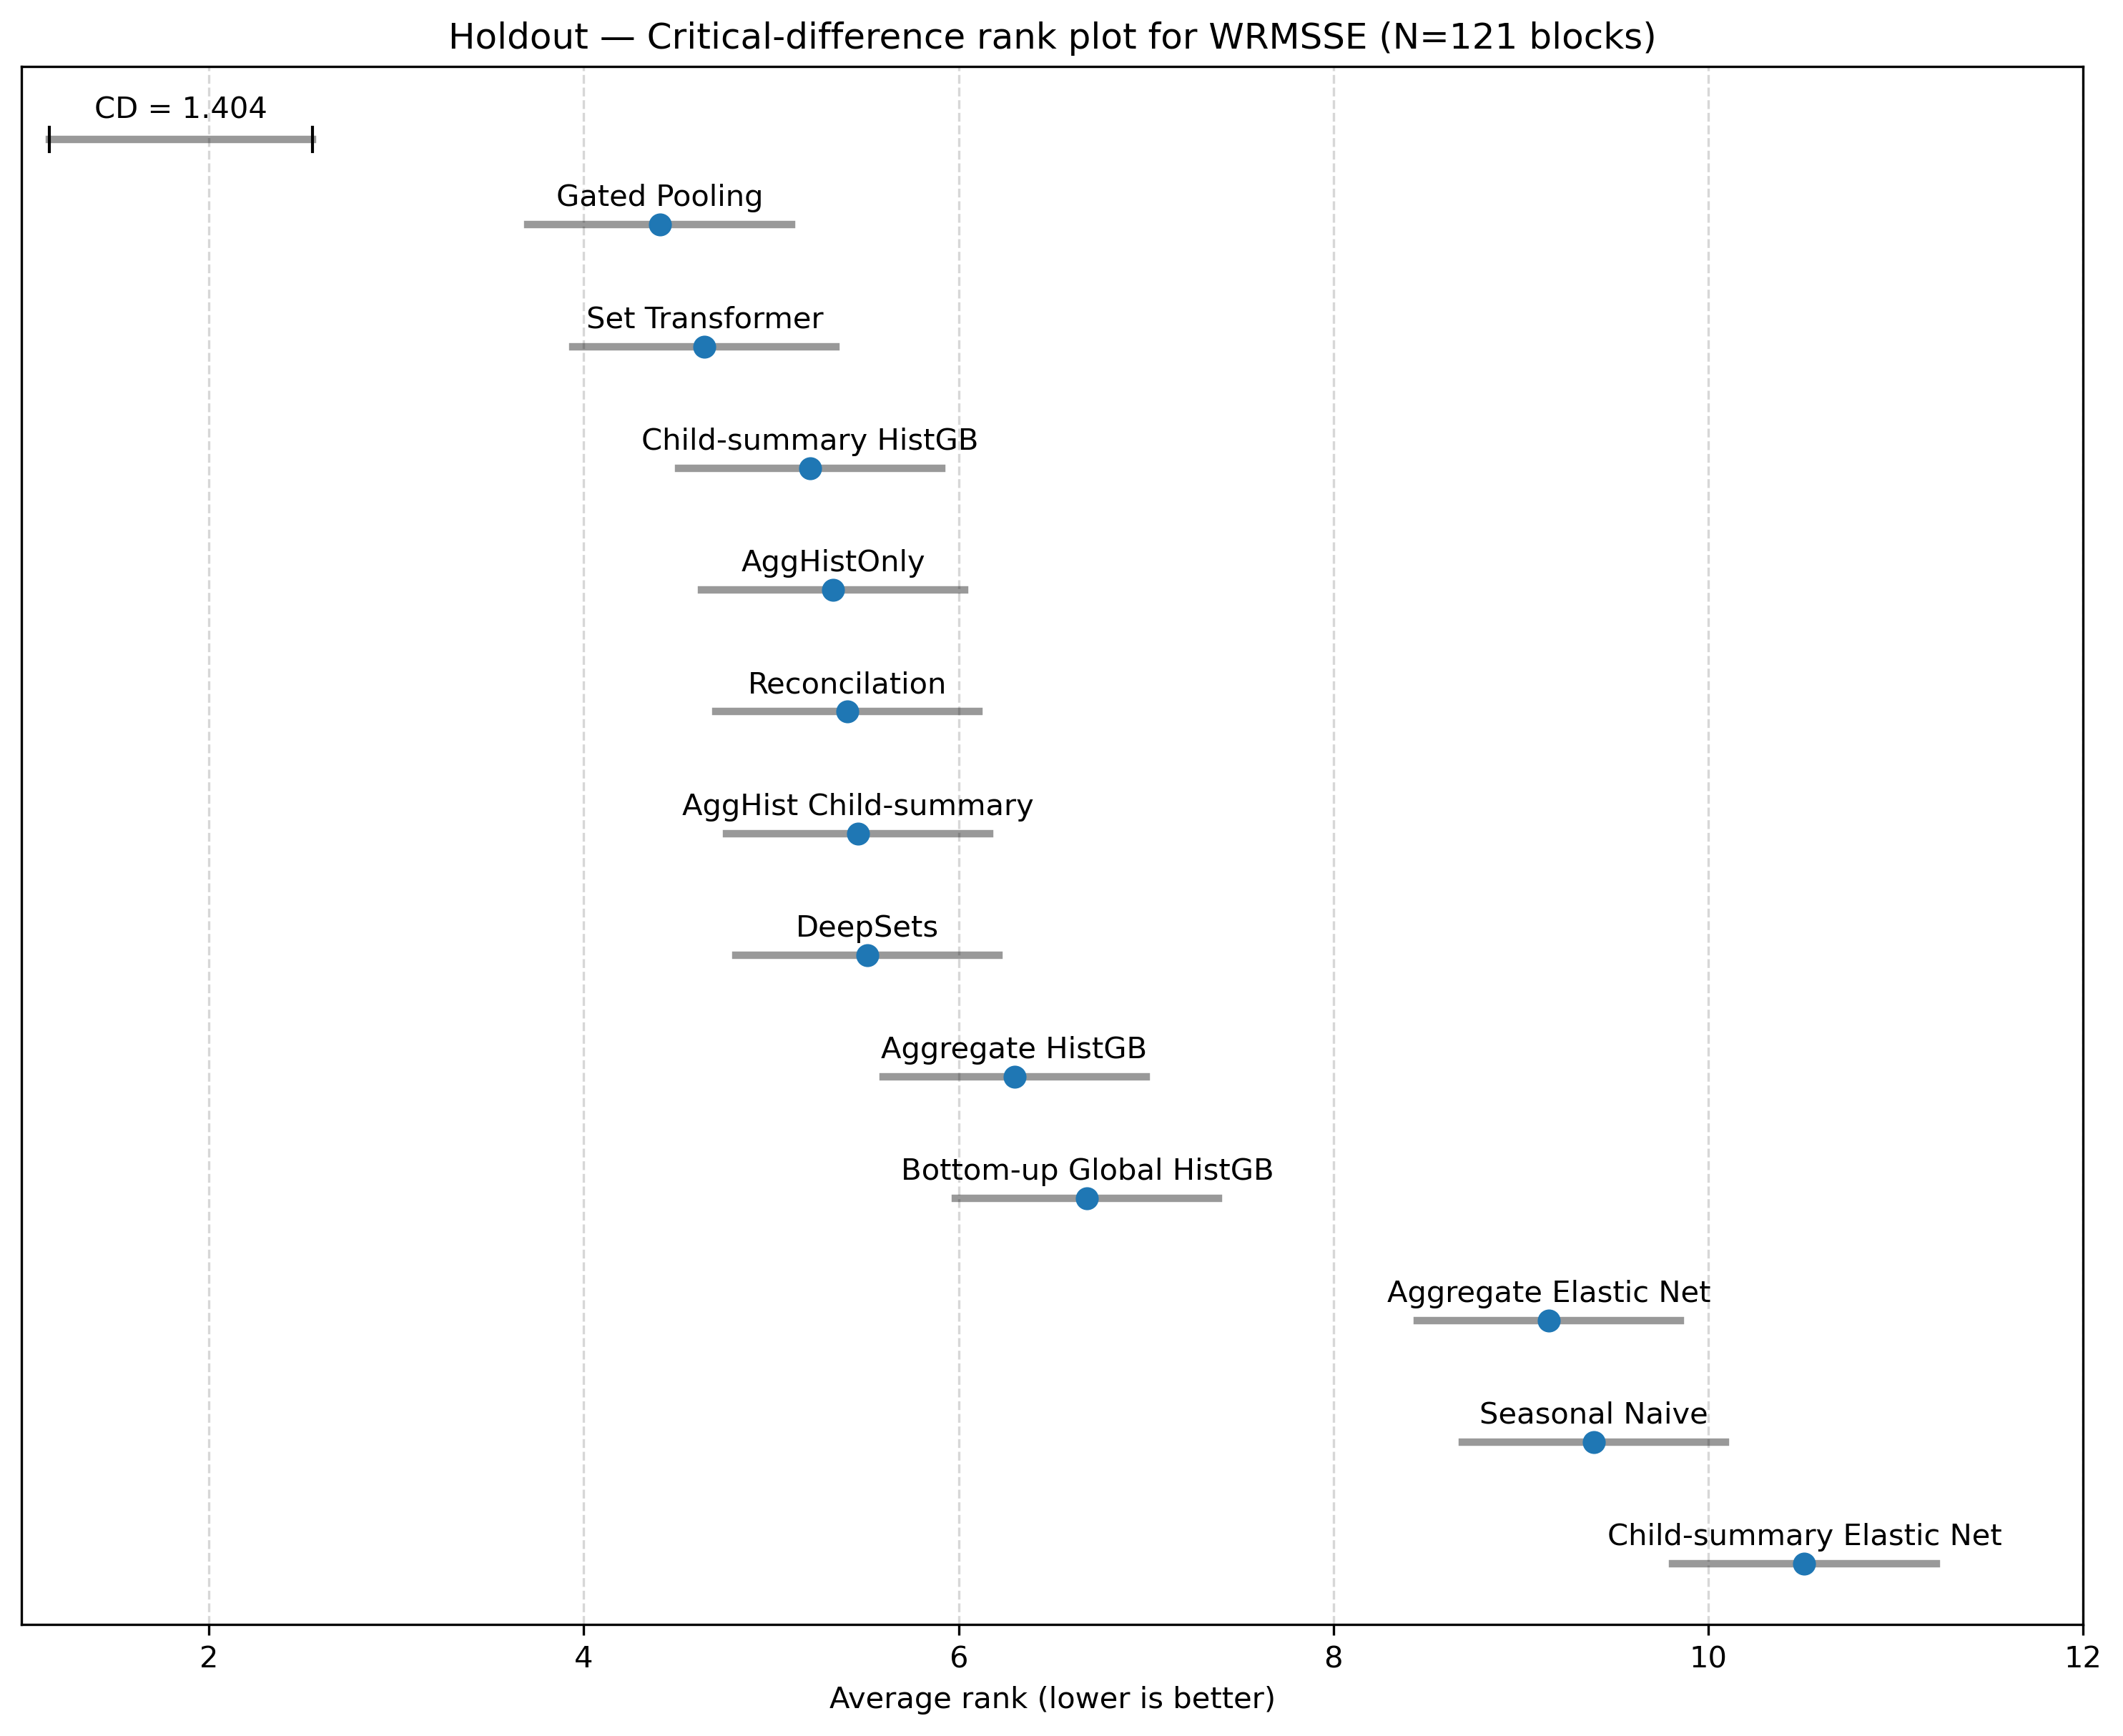
\includegraphics[width=1\textwidth]{figures/Figure_cd_diagram_wrmsse_series_holdout.png}
  \caption{Statistical comparison of point forecasting performance across aggregate series based on Friedman ranks and Nemenyi post-hoc tests. Lower average rank indicates better overall performance; connecting lines indicate groups of models whose differences are not statistically significant at $\alpha=0.1$.}
  \label{fig:point_statistical}
\end{figure}

The statistical comparison in Figure~\ref{fig:point_statistical} further strengthens the conclusions from Table~\ref{tab:main_point}. Gated Pooling achieves the best overall average rank, followed very closely by Set Transformer. Child-summary HistGB also ranks strongly, contributing to a tight leading group. The proposed learned cross-level models all achieve multiple statistically significant wins and no significant losses in the Nemenyi post-hoc comparison, indicating that their advantage is not confined to a small subset of aggregate series. By contrast, Aggregate Elastic Net, Seasonal Naive, and Child-summary Elastic Net rank clearly lower and exhibit multiple significant losses. Bottom-up Global HistGB, while competitive in raw WRMSSE, shows a more mixed ranking profile with several significant losses, suggesting that its performance advantage is less uniform across series than that of the set-based models.

It is also worth noting that Bottom-up Global HistGB performs competitively in raw WRMSSE terms, but its average rank falls clearly behind the leading group of learned models and it exhibits several statistically significant losses. This confirms that child-level information is useful for aggregate forecasting even when using bottom-up forecasting aggregation, but the learned set-based models achieve better overall ranking positions and more favorable significance outcomes, indicating that representation learning provides additional value beyond simple bottom-up summation.

\subsection{Probabilistic forecasting results}

Table~\ref{tab:main_quantile} reports the probabilistic forecasting results across the three aggregate forecasting tasks. The overall pattern is in general consistent with that observed for point forecasting. The proposed cross-level models achieve substantially lower WSPL than the direct aggregate-level baselines and the bottom-up probabilistic baselines on all three tasks, indicating that child-level information is also valuable for modeling predictive uncertainty at the aggregate level. This result is noteworthy because probabilistic forecasting is more demanding than point forecasting: the model must learn not only the conditional location of the aggregate target, but also the shape and dispersion of its predictive distribution. The lower WSPL values therefore suggest that the proposed framework is able to exploit child-level heterogeneity to better characterize aggregate uncertainty, rather than merely improving the prediction of central tendency.

\begin{table}[H]
  \centering
  \caption{Probabilistic forecasting results across aggregate forecasting tasks.}
  \label{tab:main_quantile}
  \begin{threeparttable}
    \begin{tabular}{lcccc}
      \toprule
      Model                     & state$\times$dept  & store$\times$cat   & store$\times$dept  & Mean               \\
      \midrule
      Set Transformer                   & \textbf{0.1686}    & 0.1907             & \underline{0.1949} & \textbf{0.1847}    \\
      DeepSets                  & \underline{0.1761} & \underline{0.1869} & 0.2022             & \underline{0.1884} \\
      Gated Pooling                  & 0.1858             & \underline{0.1857} & \textbf{0.1944}    & 0.1886             \\
      AggHist Child-summary   & 0.2049             & 0.1928             & 0.2120             & 0.2032             \\
      AggHistOnly               & 0.2040             & \textbf{0.1836}    & 0.2094             & 0.1990             \\
      Bottom-up Global HistGB  & 0.2081	     &0.2169	            &0.2406	             &0.2219             \\
      Aggregate Elastic Net     & 0.2526             & 0.2538             & 0.2630             & 0.2565             \\
      Child-summary Elastic Net & 0.2829             & 0.3255             & 0.2781             & 0.2955             \\
      Aggregate HistGB          & 0.2759             & 0.2545             & 0.2768             & 0.2691             \\
      Child-summary HistGB      & 0.2713             & 0.2660             & 0.2847             & 0.2740             \\
      Seasonal Naive            & 0.2677             & 0.2660             & 0.2906             & 0.2748             \\
      \bottomrule
    \end{tabular}
    \begin{tablenotes}
      \footnotesize \item Entries report WSPL. Lower values indicate better performance. The best result in each column is shown in bold, and the second-best result is underlined.
    \end{tablenotes}
  \end{threeparttable}
\end{table}


The relative ordering of the proposed models is broadly consistent with the point forecasting results, but with some task-specific variation. Set Transformer achieves the best average performance overall and attains the best result on the state$\times$department task, whereas Gated Pooling ranks first on the store$\times$category and store$\times$department tasks. DeepSets also performs competitively, ranking very close to Gated Pooling on average. All three proposed variants outperform the benchmark baselines by a clear margin. This pattern indicates that explicit set representation learning is beneficial not only for aggregate point forecasting, but also for quantile forecasting.

Figure~\ref{fig:quantile_statistical} reports the statistical comparison of probabilistic forecasting performance across 121 aggregate series. The figure summarizes the Friedman ranking results together with the Nemenyi post-hoc comparisons, thereby complementing the average WSPL values reported in Table~\ref{tab:main_quantile} with a distribution-sensitive assessment of model performance.

\begin{figure}[t]
  \centering
  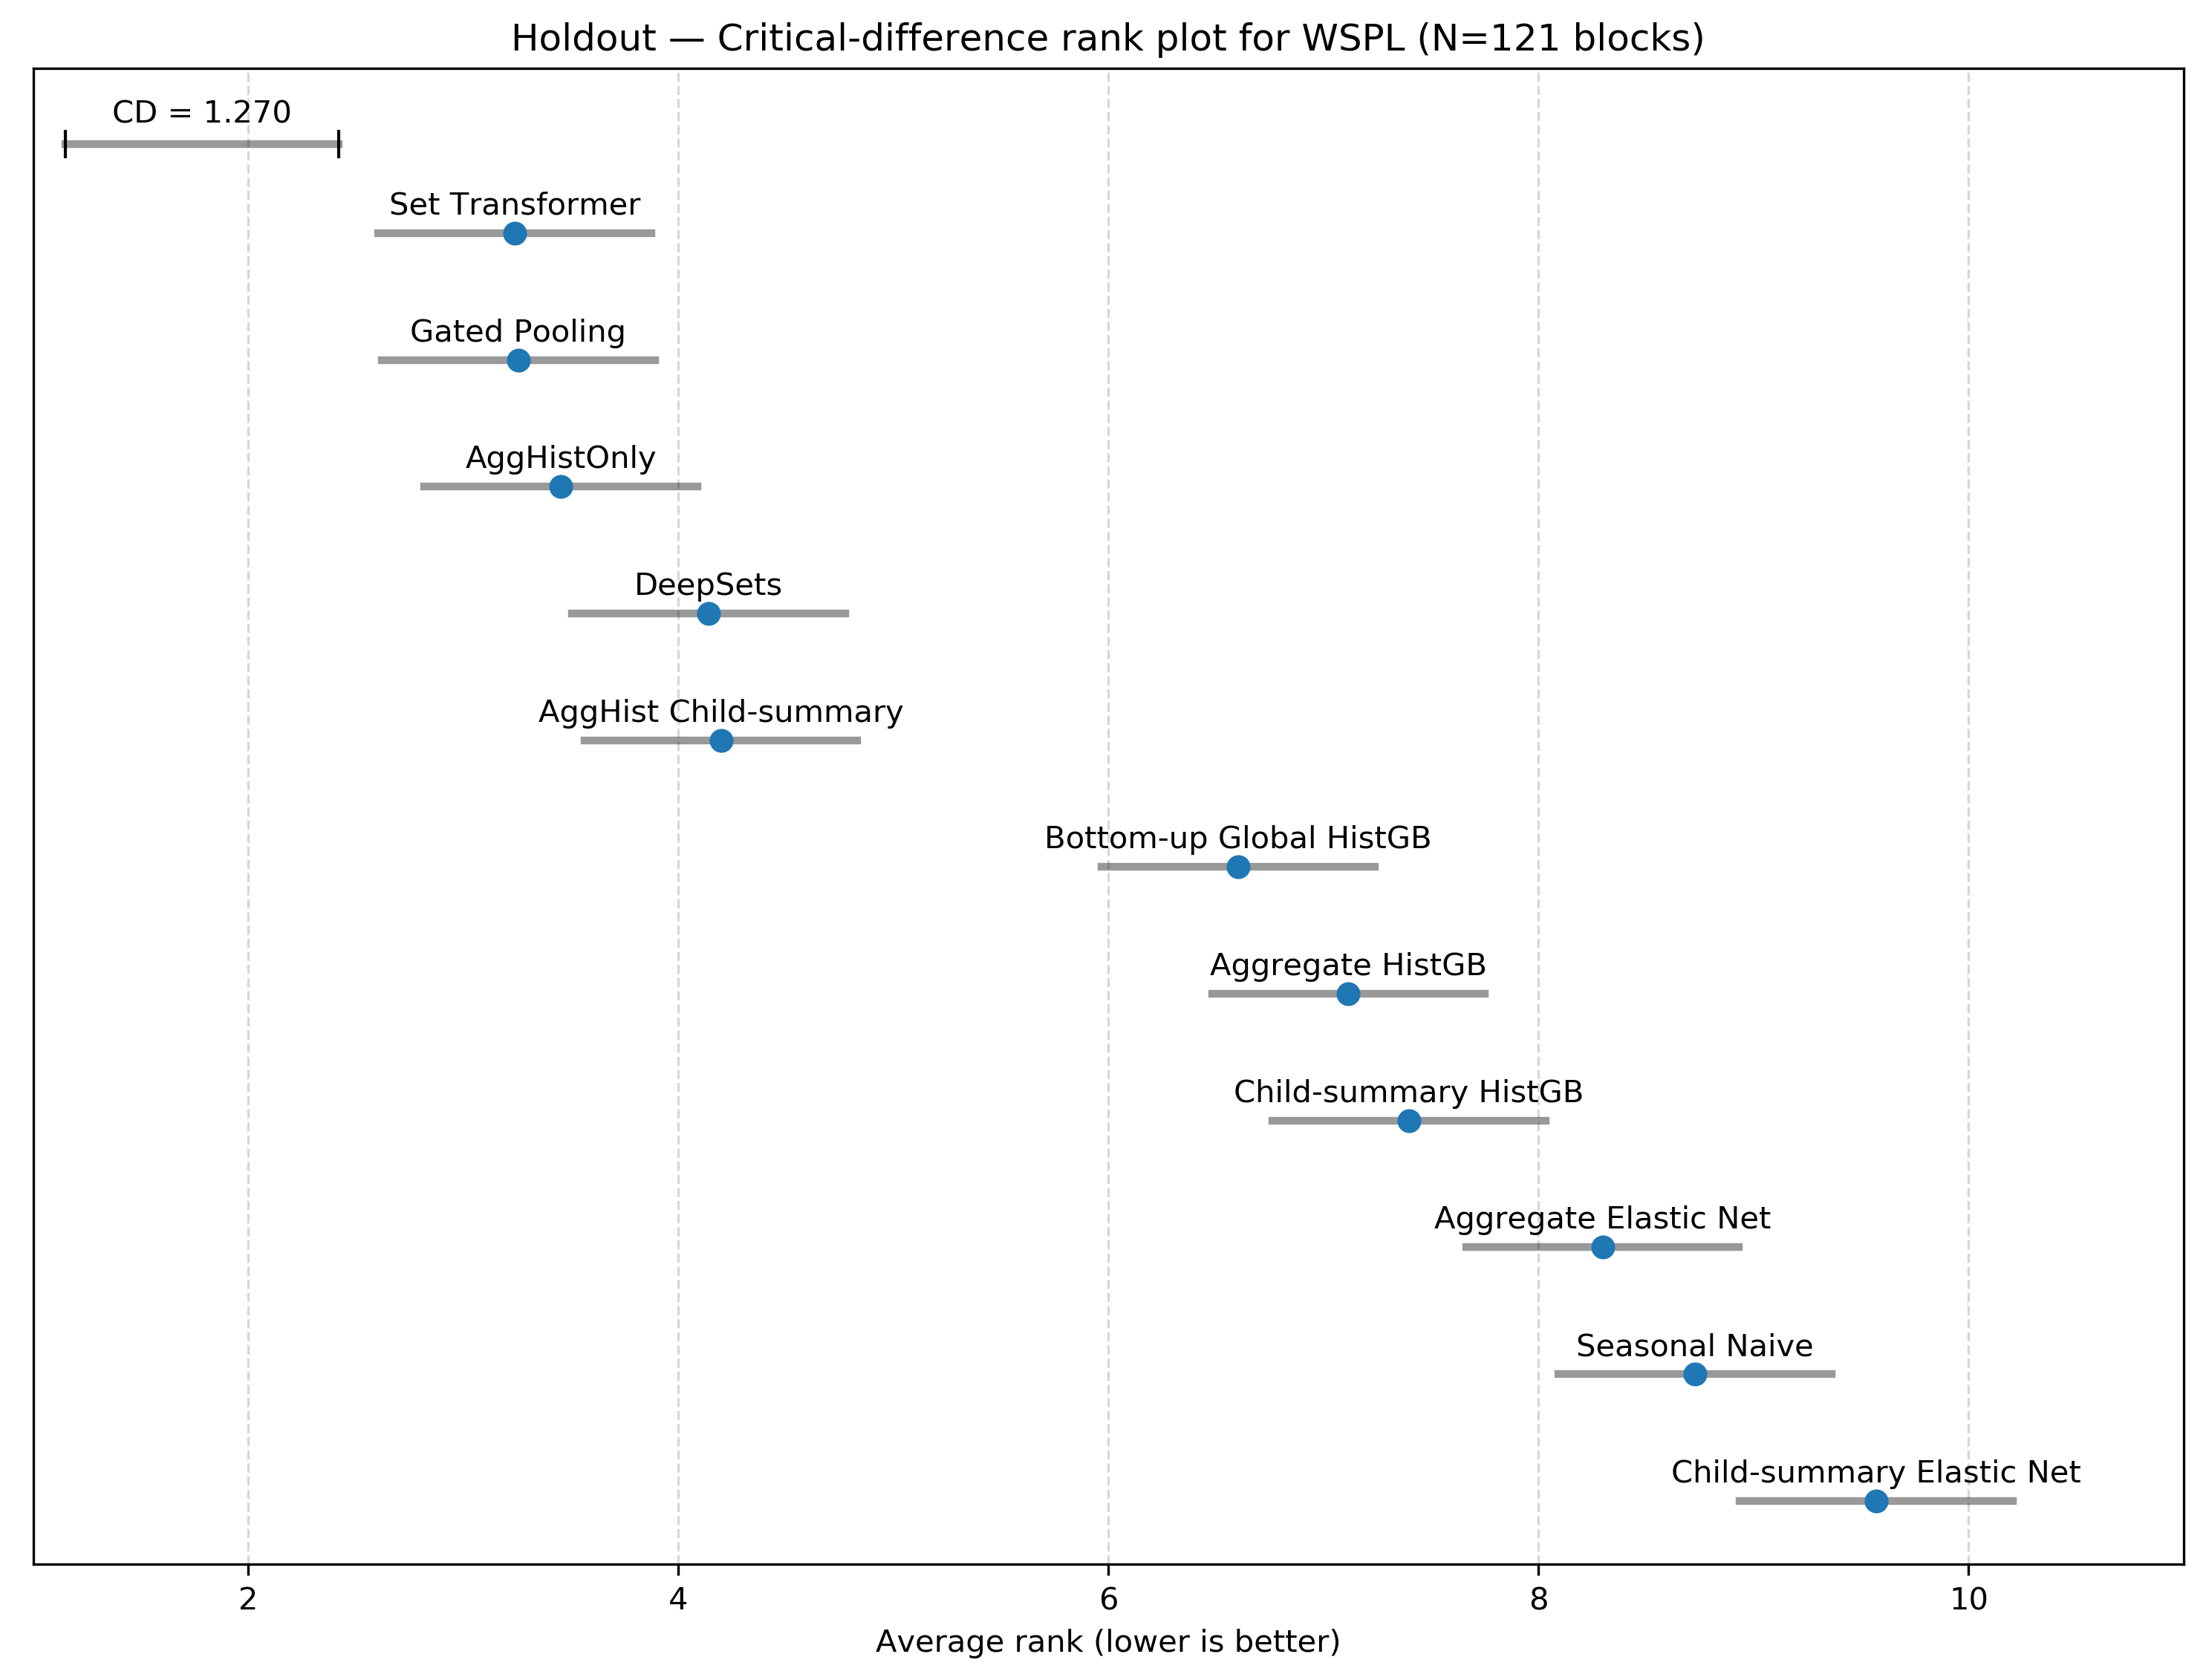
\includegraphics[width=1\textwidth]{figures/Figure_cd_diagram_mean_spl_series.png}
  \caption{Statistical comparison of quantile forecasting performance across aggregate series based on Friedman ranks and Nemenyi post-hoc tests. Lower average rank indicates better overall performance; connecting lines indicate groups of models whose differences are not statistically significant at $\alpha=0.1$.}
  \label{fig:quantile_statistical}
\end{figure}

The rank ordering in Figure~\ref{fig:quantile_statistical} is broadly consistent with, but not identical to, the mean WSPL results in Table~\ref{tab:main_quantile}. Set Transformer achieves the best average rank, followed very closely by Gated Pooling. AggHistOnly, DeepSets, and AggHist Child-summary form a tight group immediately behind the two leading models. These five models form a clear leading group, well ahead of the benchmark methods. Among the external baselines, Bottom-up Global HistGB is the strongest, followed by Aggregate HistGB and Child-summary HistGB, whereas the ElasticNet variants rank lower and Seasonal Naive performs worst by a wide margin.

\subsection{Robustness results}

\subsubsection{Rolling-origin evaluation}

Tables~\ref{tab:rolling_point} and~\ref{tab:rolling_quantile} report the detailed rolling-origin point and probabilistic forecasting results across the three aggregate forecasting tasks, while Figures~\ref{fig:rolling_point_statistical} and~\ref{fig:rolling_quantile_statistical} present the corresponding Friedman rank comparisons. The overall pattern is consistent with the holdout results, confirming that the findings are not an artifact of a particular temporal evaluation design.

\begin{table}[H]
  \centering
  \caption{Rolling-origin point forecasting results across aggregate forecasting tasks.}
  \label{tab:rolling_point}
  \begin{threeparttable}
    \begin{tabular}{lcccc}
      \toprule
      Model                     & state$\times$dept  & store$\times$cat   & store$\times$dept  & Mean               \\
      \midrule
      Set Transformer                  & \underline{0.6748} & \underline{0.6694} & \underline{0.7195} & \textbf{0.6879}    \\
      DeepSets                  & 0.7031             & \textbf{0.6549}    & 0.7341             & 0.6973             \\
      Gated Pooling                  & \textbf{0.6690}    & 0.6833             & \textbf{0.7134}    & \underline{0.6886} \\
      Bottom-up Global HistGB  & 0.7775	      & 0.7717            	& 0.8357	           & 0.7950             \\
      AggHist Child-summary   & 0.7955             & 0.7471             & 0.8009             & 0.7812             \\
      AggHistOnly               & 0.7623             & 0.7619             & 0.7882             & 0.7708             \\
      Child-summary HistGB      & 0.7306             & 0.7257             & 0.7763             & 0.7442             \\
      Aggregate HistGB          & 0.7371             & 0.7295             & 0.7904             & 0.7523             \\
      Aggregate Elastic Net     & 1.2759             & 1.2519             & 1.2035             & 1.2438             \\
      Child-summary Elastic Net & 2.1322             & 2.1201             & 1.9959             & 2.0827             \\
      Seasonal Naive            & 0.9601             & 0.9580             & 1.0073             & 0.9752             \\
      \bottomrule
    \end{tabular}
    \begin{tablenotes}
      \footnotesize \item Entries report WRMSSE averaged across rolling forecast origins. Lower values indicate better performance. The best result in each column is shown in bold, and the second-best result is underlined.
    \end{tablenotes}
  \end{threeparttable}
\end{table}

\begin{figure}[t]
  \centering
  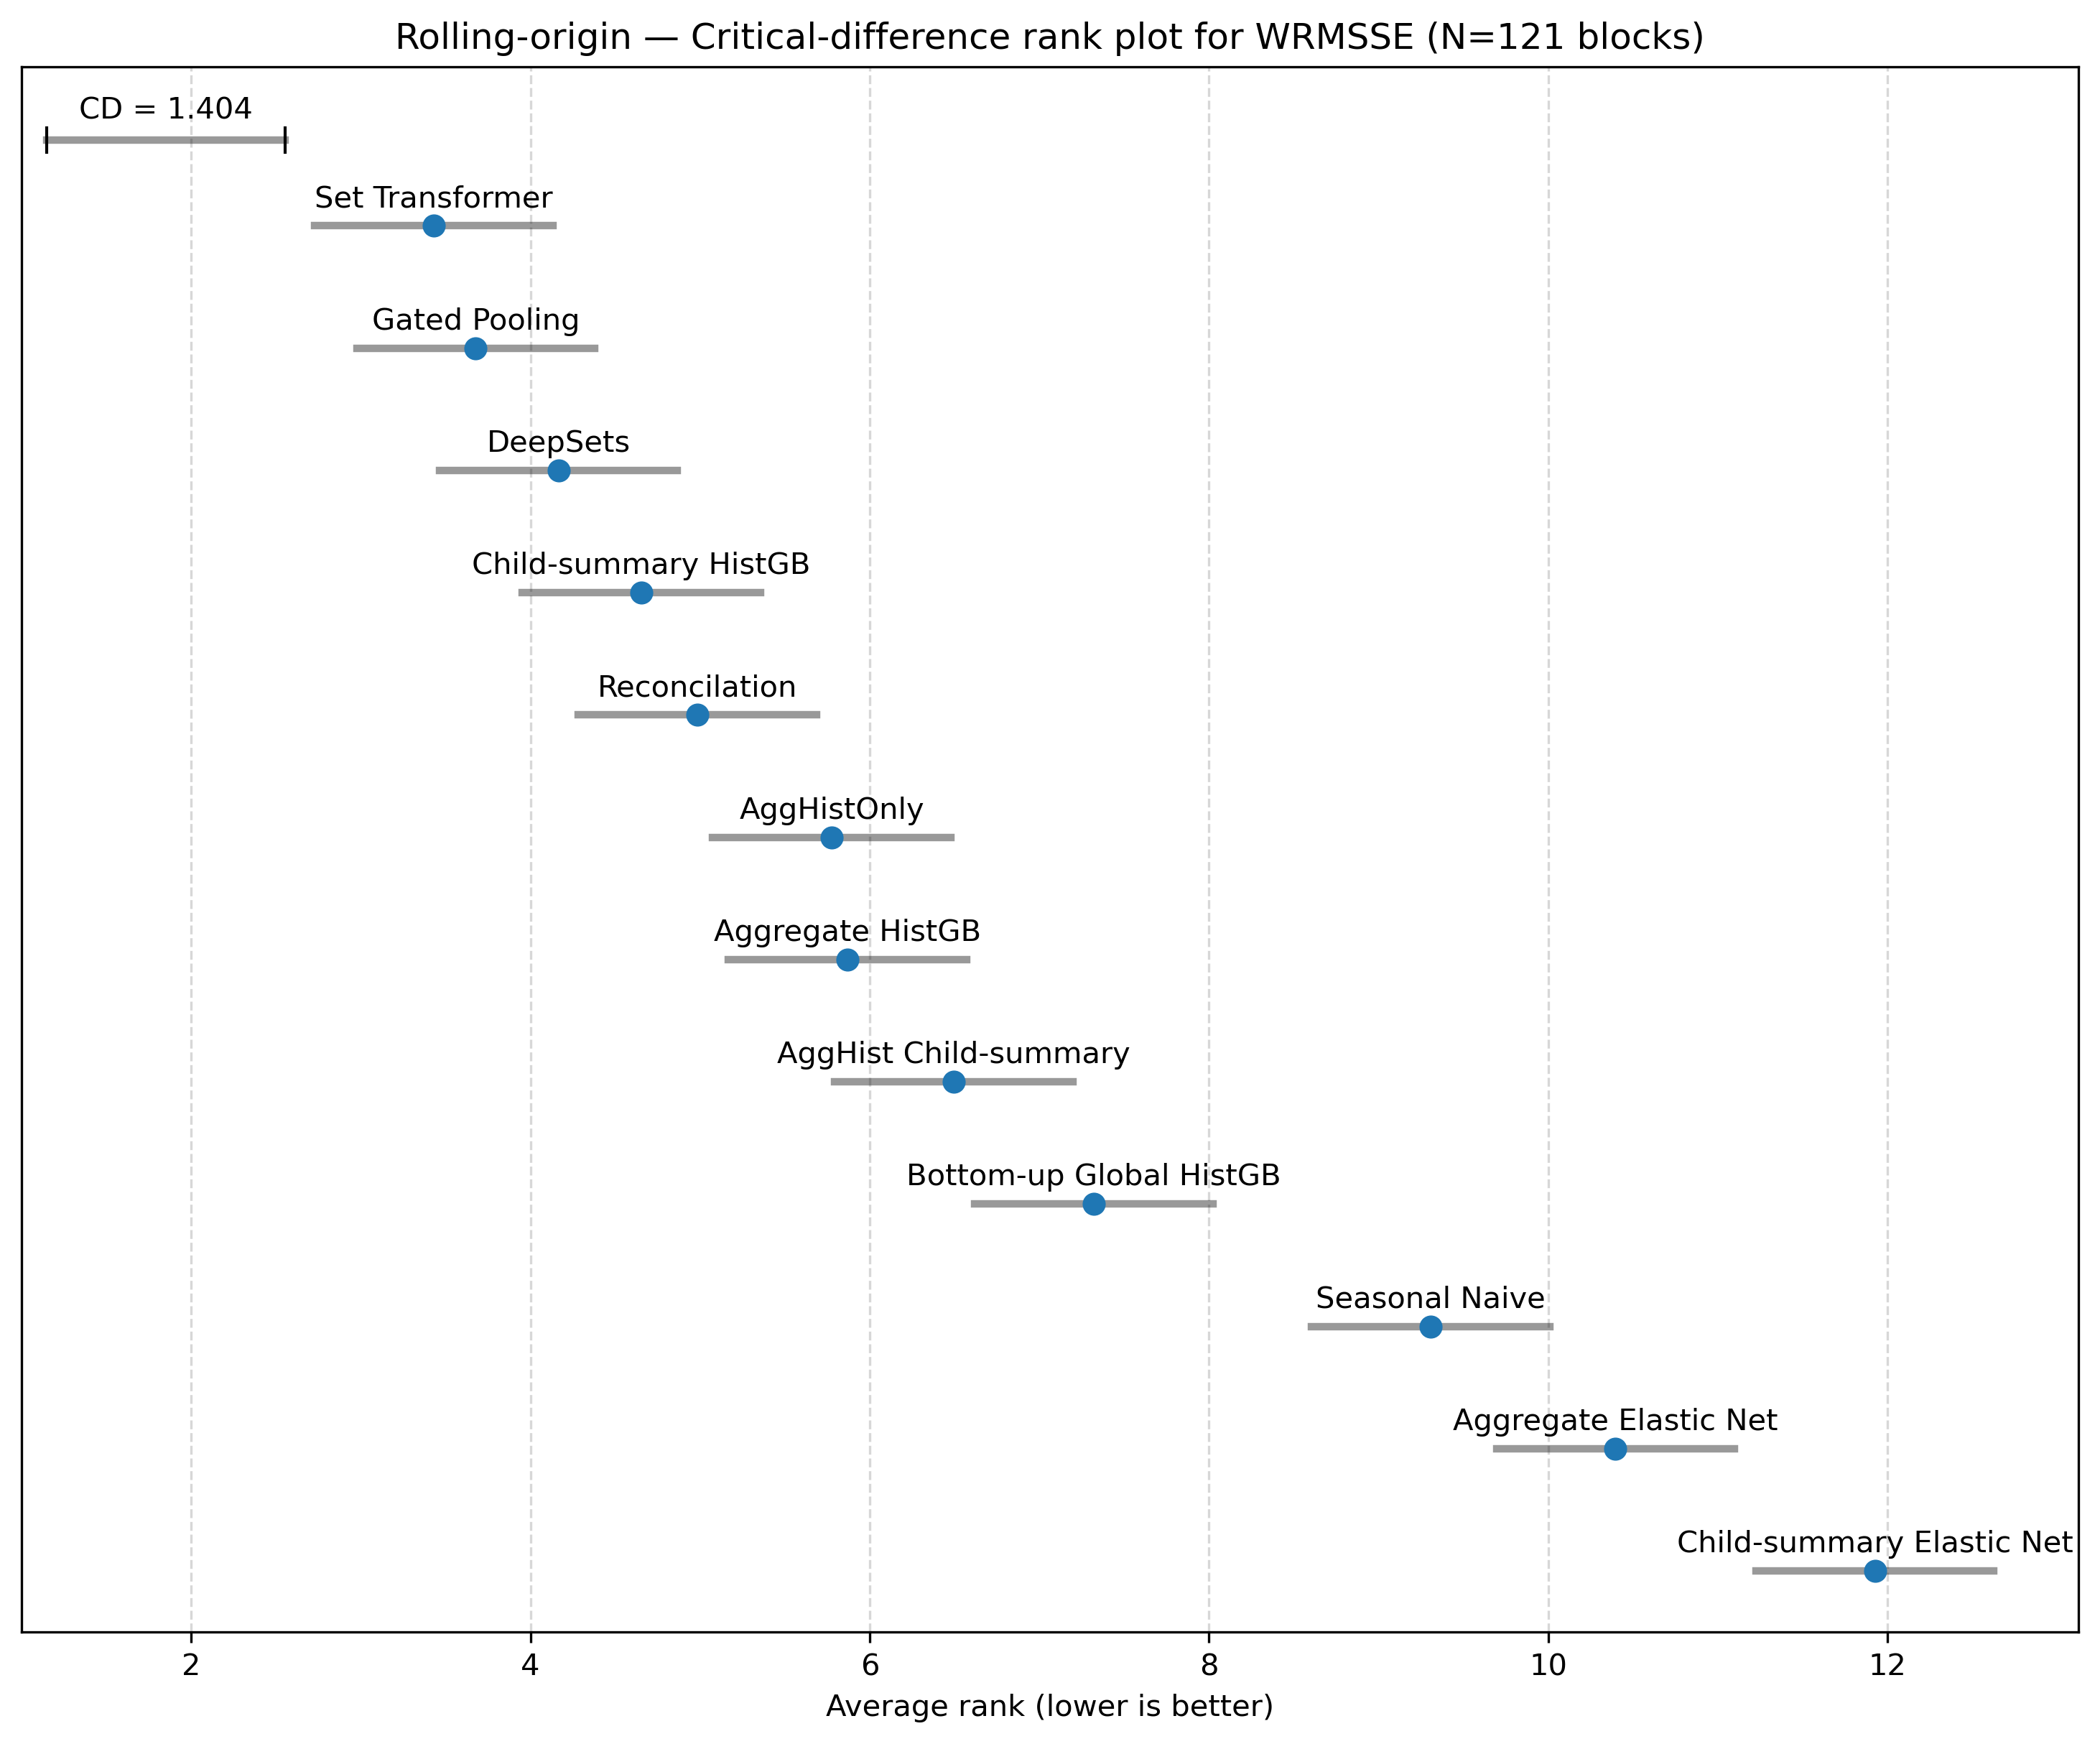
\includegraphics[width=1\textwidth]{figures/Figure_cd_diagram_wrmsse_series_rolling.png}
  \caption{Statistical comparison of rolling-origin point forecasting performance across aggregate series based on Friedman ranks and Nemenyi post-hoc tests. Lower average rank indicates better overall performance; connecting lines indicate groups of models whose differences are not statistically significant at $\alpha=0.1$.}
  \label{fig:rolling_point_statistical}
\end{figure}

\begin{table}[H]
  \centering
  \caption{Rolling-origin probabilistic forecasting results across aggregate forecasting tasks.}
  \label{tab:rolling_quantile}
  \begin{threeparttable}
    \begin{tabular}{lcccc}
      \toprule
      Model                     & state$\times$dept  & store$\times$cat   & store$\times$dept  & Mean               \\
      \midrule
      Set Transformer                   & \underline{0.1739} & \underline{0.1754} & \textbf{0.1811}    & \textbf{0.1768}    \\
      DeepSets                  & \textbf{0.1727}    & \textbf{0.1733}    & \underline{0.1849} & \underline{0.1770} \\
      Gated Pooling                  & 0.1741             & 0.1763             & 0.1885             & 0.1796             \\
      AggHist Child-summary   & 0.1995             & 0.1920             & 0.2024             & 0.1980             \\
      AggHistOnly               & 0.2052             & 0.1931             & 0.2057             & 0.2014             \\
      Bottom-up Global HistGB  & 0.2183	     &0.2188	            &0.2410	             &0.2260             \\
      Aggregate Elastic Net     & 0.3688             & 0.3620             & 0.3395             & 0.3568             \\
      Child-summary Elastic Net & 0.7215             & 0.7265             & 0.6362             & 0.6947             \\
      Aggregate HistGB          & 0.2528             & 0.2493             & 0.2585             & 0.2535             \\
      Child-summary HistGB      & 0.2605             & 0.2613             & 0.2628             & 0.2616             \\
      Seasonal Naive            & 0.2893             & 0.2862             & 0.3055             & 0.2937             \\
      \bottomrule
    \end{tabular}
    \begin{tablenotes}
      \footnotesize \item Entries report WSPL averaged across rolling forecast origins. Lower values indicate better performance. The best result in each column is shown in bold, and the second-best result is underlined.
    \end{tablenotes}
  \end{threeparttable}
\end{table}

\begin{figure}[t]
  \centering
  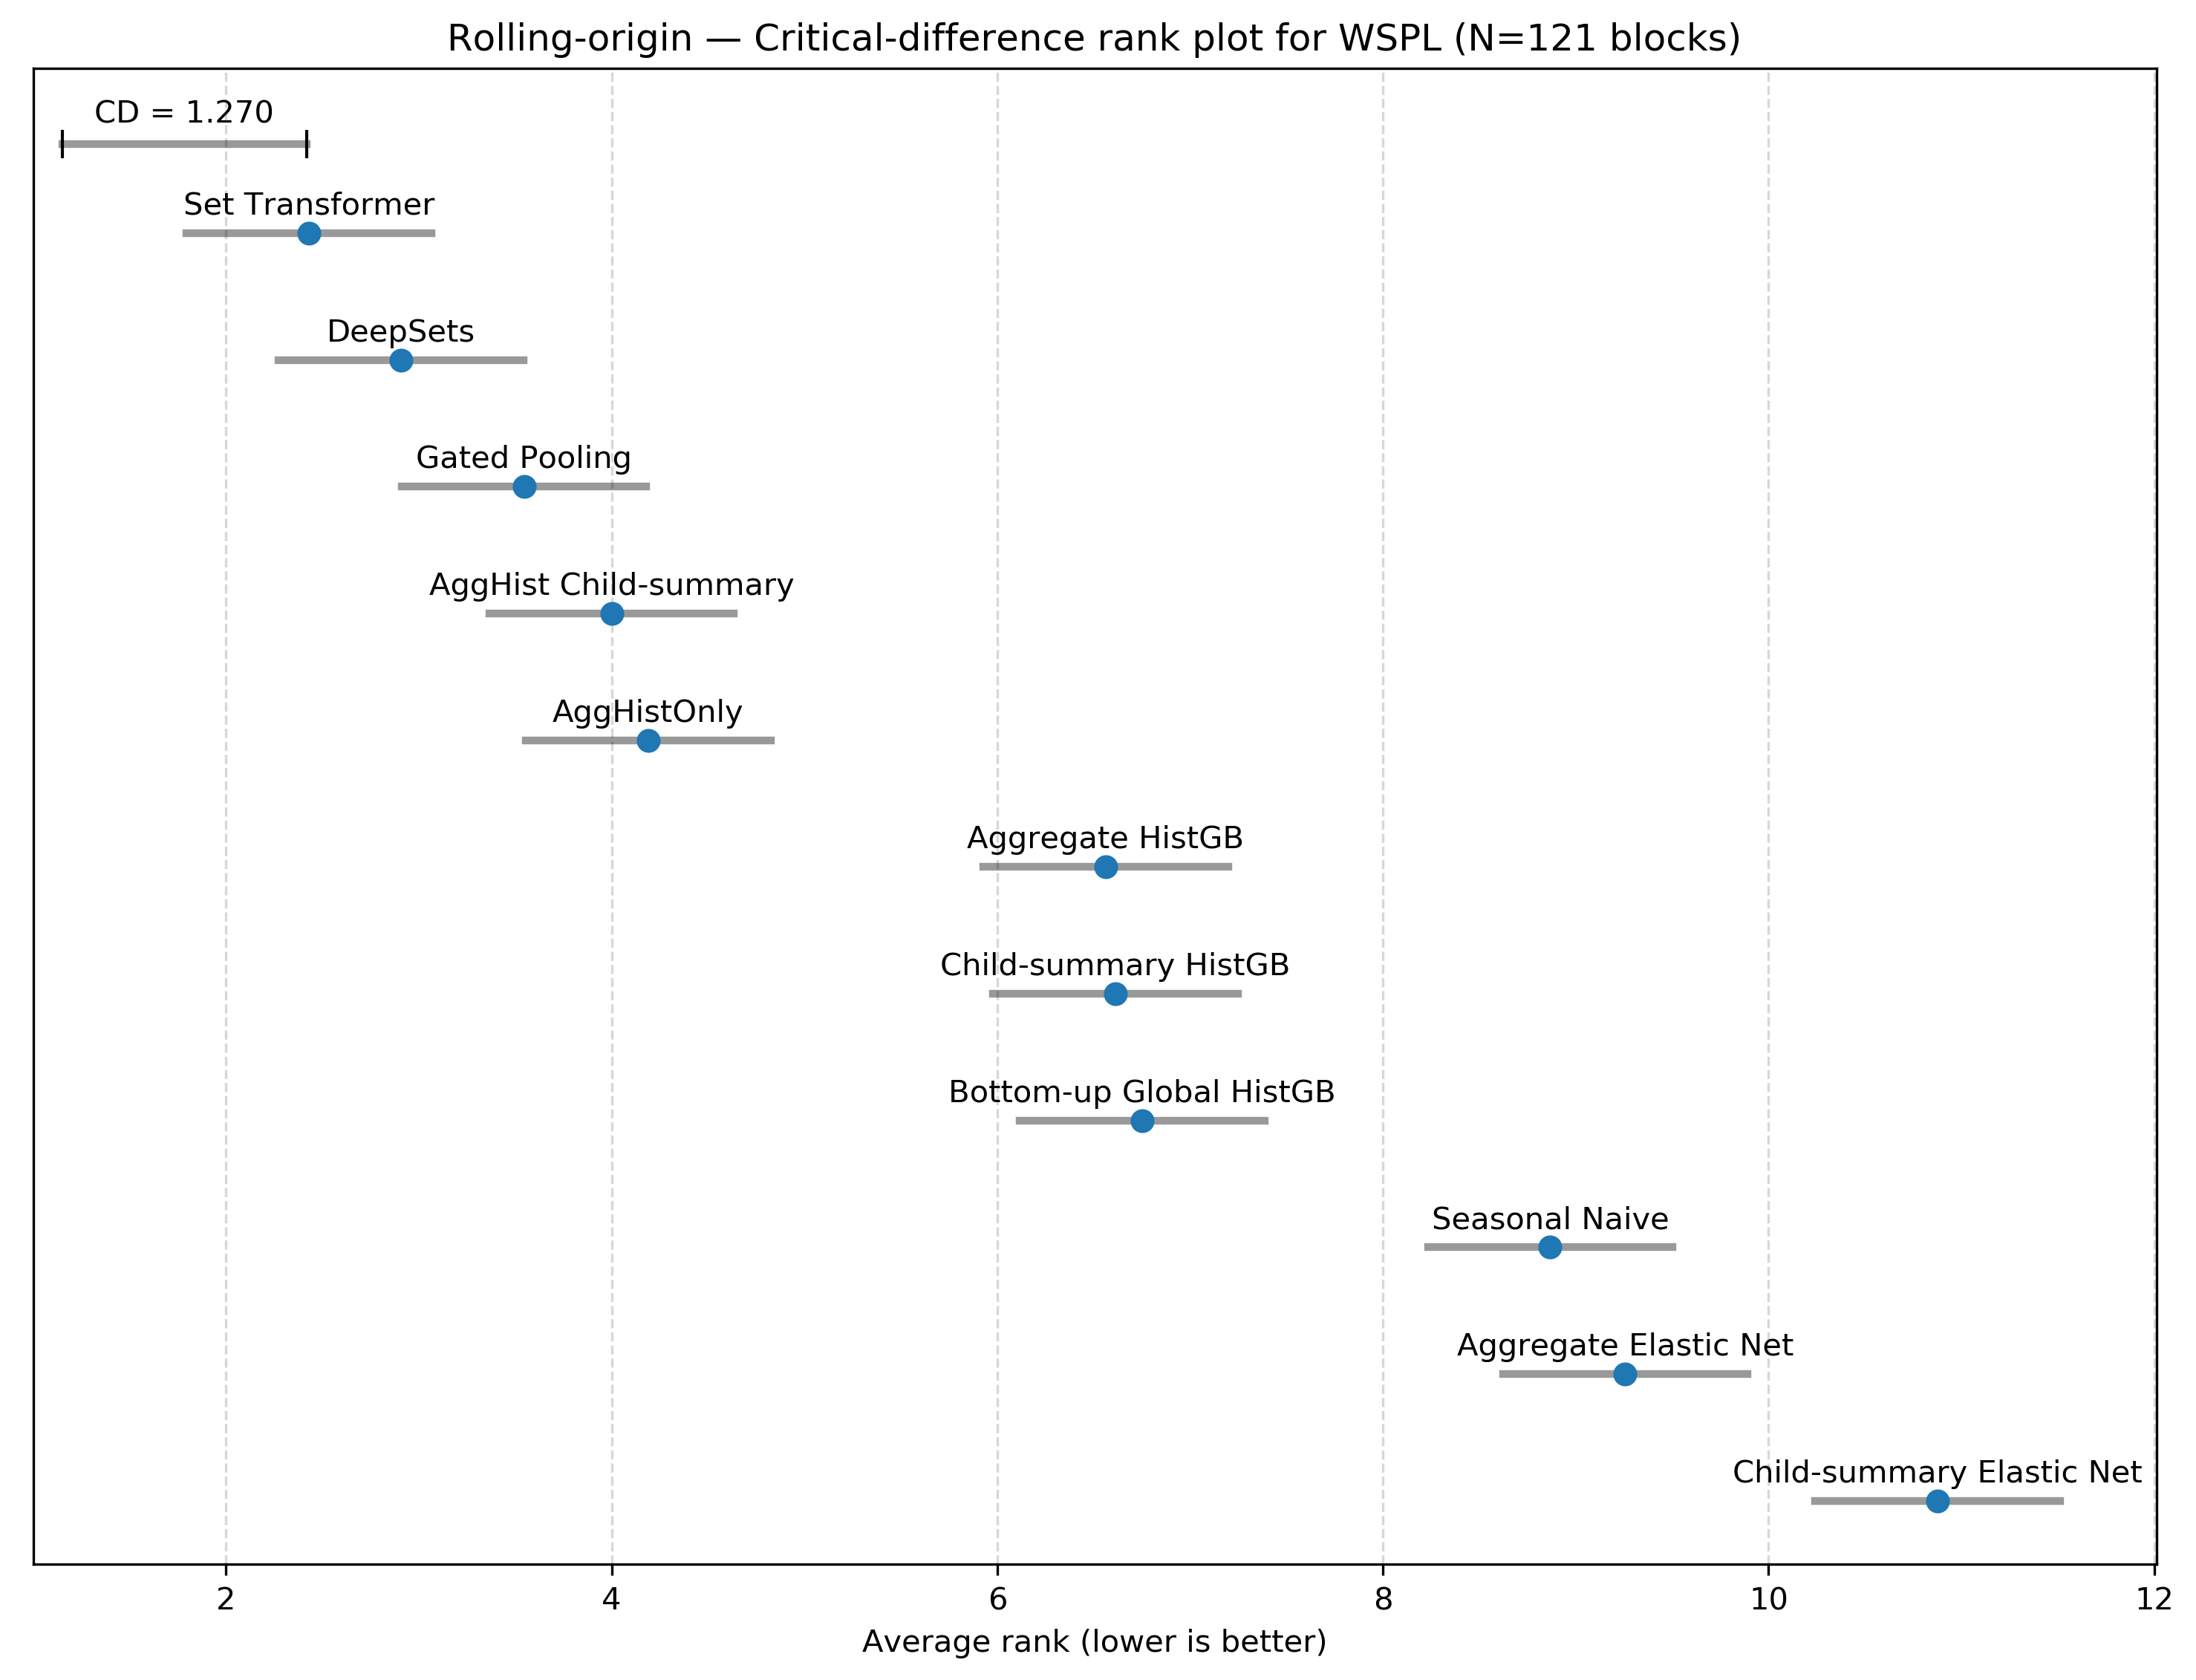
\includegraphics[width=1\textwidth]{figures/Figure_cd_diagram_mean_spl_series_rolling.png}
  \caption{Statistical comparison of rolling-origin quantile forecasting performance across aggregate series based on Friedman ranks and Nemenyi post-hoc tests. Lower average rank indicates better overall performance; connecting lines indicate groups of models whose differences are not statistically significant at $\alpha=0.1$.}
  \label{fig:rolling_quantile_statistical}
\end{figure}

In the rolling-origin point forecasting results (Table~\ref{tab:rolling_point}), Gated Pooling achieves the best per-task results on state$\times$department and store$\times$department, while DeepSets performs best on store$\times$category. Set Transformer leads the overall mean with a narrow margin over Gated Pooling. The Friedman rank comparison (Figure~\ref{fig:rolling_point_statistical}) shows Set Transformer and Gated Pooling forming a clear leading group, with DeepSets also performing competitively. For quantile forecasting (Table~\ref{tab:rolling_quantile}), DeepSets attains the best results on state$\times$department and store$\times$category, while Set Transformer leads on store$\times$department and on overall mean. The corresponding CD diagram (Figure~\ref{fig:rolling_quantile_statistical}) confirms that Set Transformer, DeepSets, and Gated Pooling form the top tier, with Set Transformer achieving the best average rank. Taken together, these rolling-origin results confirm that the advantage of the proposed set-based cross-level models is not driven by a particular test period and holds under a multi-origin temporal evaluation protocol.

\subsubsection{Sample fraction robustness}

Tables~\ref{tab:summary_point_sample_frac} and~\ref{tab:summary_quantile_sample_frac} summarize the overall mean point and probabilistic forecasting performance across the four SKU sample fractions (10\%, 30\%, 50\%, and 100\%). Several patterns emerge. First, all three proposed set-based models show a clear tendency toward better performance as the sample fraction increases, with the gains being most pronounced between 10\% and 100\%. Set Transformer and Gated Pooling benefit the most from the larger sample, while DeepSets exhibits a more gradual improvement in point forecasting but strong gains in quantile forecasting. Second, the benchmark methods generally show smaller or inconsistent improvements with larger sample fractions; Aggregate Elastic Net and Child-summary Elastic Net even degrade slightly as the sample fraction grows, likely reflecting the difficulty of linear models in exploiting richer but more heterogeneous SKU-level structure. Third, the ablation variants AggHistOnly and AggHist Child-summary also benefit from larger samples but remain consistently behind the proposed set-based models at every fraction, confirming that the set-based representation learning mechanism itself, rather than merely having access to more child-level information, drives the improvement. Detailed per-task results for the 10\%, 30\%, and 50\% fractions are reported in Appendix Tables~\ref{tab:appendix_point_10pct}--\ref{tab:appendix_quantile_50pct}.

\begin{table}[H]
  \centering
  \caption{Point forecasting results (mean WRMSSE) across SKU sample fractions.}
  \label{tab:summary_point_sample_frac}
  \begin{threeparttable}
    \begin{tabular}{lcccc}
      \toprule
      Model                     & 10\%                & 30\%                & 50\%                & 100\%               \\
      \midrule
      Set Transformer                & 0.7927 & 0.7272 & 0.7236 & 0.6897 \\
      DeepSets                       & 0.7806 & 0.7952 & 0.7233 & 0.7254 \\
      Gated Pooling                  & 0.8059 & 0.7416 & 0.7440 & 0.6938 \\
      Bottom-up Global HistGB        & 0.7978 & 0.7902 & 0.7695 & 0.7558 \\
      AggHistOnly                    & 0.8137 & 0.8056 & 0.8111 & 0.7523 \\
      AggHist Child-summary          & 0.8163 & 0.7972 & 0.7776 & 0.7641 \\
      Child-summary HistGB           & 0.8107 & 0.7778 & 0.7498 & 0.7467 \\
      Aggregate HistGB               & 0.8285 & 0.8038 & 0.7670 & 0.7595 \\
      Seasonal Naive                 & 0.9757 & 0.9356 & 0.9148 & 0.9137 \\
      Aggregate Elastic Net          & 0.9126 & 0.9243 & 0.9389 & 0.9437 \\
      Child-summary Elastic Net      & 0.9613 & 1.0054 & 1.0190 & 1.0759 \\
      \bottomrule
    \end{tabular}
    \begin{tablenotes}
      \footnotesize \item Entries report the overall mean WRMSSE across the three aggregate forecasting tasks (state$\times$department, store$\times$category, store$\times$department). Lower values indicate better performance. Each column corresponds to a different random sampling fraction of the bottom-level SKU--store series.
    \end{tablenotes}
  \end{threeparttable}
\end{table}

\begin{table}[H]
  \centering
  \caption{Probabilistic forecasting results (mean WSPL) across SKU sample fractions.}
  \label{tab:summary_quantile_sample_frac}
  \begin{threeparttable}
    \begin{tabular}{lcccc}
      \toprule
      Model                     & 10\%                & 30\%                & 50\%                & 100\%               \\
      \midrule
      Set Transformer                & 0.1947 & 0.1926 & 0.1933 & 0.1847 \\
      DeepSets                       & 0.1956 & 0.1936 & 0.1886 & 0.1884 \\
      Gated Pooling                  & 0.1993 & 0.1947 & 0.1949 & 0.1886 \\
      Bottom-up Global HistGB        & 0.2257 & 0.2281 & 0.2242 & 0.2219 \\
      AggHistOnly                    & 0.2096 & 0.2088 & 0.2142 & 0.1990 \\
      AggHist Child-summary          & 0.2103 & 0.2059 & 0.2041 & 0.2032 \\
      Aggregate HistGB               & 0.2639 & 0.2727 & 0.2652 & 0.2691 \\
      Child-summary HistGB           & 0.2654 & 0.2737 & 0.2705 & 0.2740 \\
      Seasonal Naive                 & 0.2773 & 0.2743 & 0.2714 & 0.2748 \\
      Aggregate Elastic Net          & 0.2466 & 0.2514 & 0.2559 & 0.2565 \\
      Child-summary Elastic Net      & 0.2577 & 0.2730 & 0.2774 & 0.2955 \\
      \bottomrule
    \end{tabular}
    \begin{tablenotes}
      \footnotesize \item Entries report the overall mean WSPL across the three aggregate forecasting tasks (state$\times$department, store$\times$category, store$\times$department). Lower values indicate better performance. Each column corresponds to a different random sampling fraction of the bottom-level SKU--store series.
    \end{tablenotes}
  \end{threeparttable}
\end{table}


\subsection{Discussion}

Taken together, the results provide clear support for the main hypothesis of the paper. Aggregate retail forecasting can benefit from child-SKU information, provided that this information is incorporated through a representation learning mechanism that respects the set structure of child units. Direct aggregate-level models do not fully exploit such information, while handcrafted child summaries only partially do so. The proposed set-based models provide a more effective way to bridge the mismatch between target granularity and information granularity.

At the same time, the results reveal a more nuanced pattern than a simple superiority claim for any single architecture. Across both point forecasting and probabilistic forecasting, Set Transformer delivers the strongest average performance overall. Gated Pooling performs very closely in both point and quantile forecasting and attains the best rank in the point forecasting statistical comparison as well as the best per-task results on store$\times$department. DeepSets also performs competitively in quantile forecasting, though its average rank falls behind the leading group in the Friedman comparison. The ablation variant AggHistOnly shows surprisingly strong ranking performance, particularly in the quantile setting, which warrants further investigation. All three proposed variants improve substantially over the external baselines and the ablation variants, showing that explicit encoding of child-level future trajectories and learned cross-SKU aggregation both contribute meaningful value. These findings suggest that the main source of improvement lies first in exploiting fine-grained child-level information, and second in aggregating it through a learned child-to-aggregate representation.

The results also indicate that the gains from cross-level representation learning are task-dependent. They are most pronounced at the more aggregated forecasting levels, especially state$\times$department and, to a slightly lesser extent, store$\times$category. By contrast, at store$\times$department level, where the target is closer to the child level, the gains remain positive but are relatively smaller.

Finally, the empirical evidence also points to an important practical caution. More flexible cross-level models do not automatically guarantee better results in all settings. Although Set Transformer is the strongest overall model in the present study, Gated Pooling performs very closely and even surpasses it in the point forecasting rank comparison and on several individual tasks, suggesting that simpler learned weighting mechanisms can be highly effective when the full SKU set is observed. 

\section{Conclusion}
\label{sec:conclusion}

This paper studied a cross-level retail forecasting problem in which the prediction target is defined at an aggregate level, while the informative explanatory variables originate at SKU level. This mismatch between target granularity and information granularity is common in retail operations, yet it is not fully addressed by either conventional aggregate-level forecasting or hierarchical forecasting methods. Direct aggregate-level models may lose important predictive information when child-level variables are simply averaged or summed. Bottom-up approaches preserve child-level detail but do not explicitly learn a representation optimized for aggregate forecasting. To address this gap, we proposed a set-based cross-level forecasting framework that first learns child-SKU temporal representations and then aggregates them through set-based encoders to generate forecasts directly at the aggregate level.

The empirical results on M5 dataset support the main premise of the study. First, fine-grained SKU-level information can improve aggregate retail sales forecasting when it is incorporated through the proposed representation learning framework. Second, the gain does not arise merely from including more variables. Models based on learned set representations outperform benchmarks that use direct aggregate modeling or handcrafted summaries of SKU-level variables. Third, among the proposed variants, Set Transformer achieves the strongest overall performance, while Gated Pooling performs very closely and attains the best results on several tasks and in the point forecasting rank comparison. DeepSets also offers a competitive alternative, particularly in quantile forecasting. Fourth, these conclusions extend beyond point forecasting and are also reflected in probabilistic forecasting performance.

The paper contributes to the forecasting literature by framing aggregate retail forecasting with child-level explanatory information as a cross-level representation learning problem. This perspective is distinct from the usual concerns of forecast reconciliation or coherence across hierarchical levels. The key challenge here is not how to maintain consistency across levels, but how to preserve fine-grained predictive signals when the target is defined at an aggregated node. By introducing set-based representation learning into this setting, the paper provides a modeling framework that is naturally suited to variable-size, unordered child collections and that can be adapted to other retail and operations settings with similar structural characteristics.

Several limitations of the present study should also be acknowledged. First, the empirical analysis is based on a single benchmark dataset, although it is a large and widely used one. Additional evidence from other retail settings would help assess the generality of the findings. Second, the current framework does not explicitly model cross-aggregate dependencies, such as interactions across stores or regions, which may also matter in practice. Third, although the paper compares three cross-level aggregation mechanisms, other forms of representation learning may also prove promising.

These limitations point naturally to several directions for future research. One direction is to extend the framework to richer multi-level settings that combine cross-level representation learning with hierarchical coherence constraints. Another is to integrate explicit graph or relation structures among child SKUs, which may allow the model to better capture substitution and complementarity effects. A third direction is to study the operational value of aggregate forecasts produced by cross-level models in downstream decision problems, such as category-level replenishment, pricing, or promotional planning. More broadly, future work may explore whether the same cross-level representation learning principle can be applied in other business forecasting settings where targets and explanatory information are observed at different granularities.

\printbibliography

\clearpage
\subsection{Detailed results by SKU sample fraction}

\begin{table}[H]
  \centering
  \caption{Point forecasting results with 10\% SKU sample.}
  \label{tab:appendix_point_10pct}
  \begin{threeparttable}
    \begin{tabular}{lcccc}
      \toprule
      Model                     & state$\times$dept  & store$\times$cat   & store$\times$dept  & Mean               \\
      \midrule
      Set Transformer                & 0.7788             & \textbf{0.7653}    & \underline{0.8339} & \underline{0.7927} \\
      DeepSets                       & \textbf{0.7432}    & 0.7820             & \textbf{0.8165}    & \textbf{0.7806}    \\
      Gated Pooling                  & 0.7848             & \underline{0.7675} & 0.8653             & 0.8059             \\
      Bottom-up Global HistGB        & \underline{0.7715} & 0.7816             & 0.8403             & 0.7978             \\
      AggHistOnly                    & 0.7754             & 0.8193             & 0.8465             & 0.8137             \\
      AggHist Child-summary          & 0.7904             & 0.8199             & 0.8385             & 0.8163             \\
      Child-summary HistGB           & 0.7770             & 0.8118             & 0.8434             & 0.8107             \\
      Aggregate HistGB               & 0.8007             & 0.8340             & 0.8508             & 0.8285             \\
      Aggregate Elastic Net          & 0.9268             & 0.8970             & 0.9139             & 0.9126             \\
      Child-summary Elastic Net      & 1.0126             & 0.9320             & 0.9392             & 0.9613             \\
      Seasonal Naive                 & 0.9326             & 0.9685             & 1.0261             & 0.9757             \\
      \bottomrule
    \end{tabular}
    \begin{tablenotes}
      \footnotesize \item Entries report WRMSSE with 10\% SKU--store series sampled. Lower values indicate better performance. Best results are shown in bold and second-best results are underlined.
    \end{tablenotes}
  \end{threeparttable}
\end{table}

\begin{table}[H]
  \centering
  \caption{Point forecasting results with 30\% SKU sample.}
  \label{tab:appendix_point_30pct}
  \begin{threeparttable}
    \begin{tabular}{lcccc}
      \toprule
      Model                     & state$\times$dept  & store$\times$cat   & store$\times$dept  & Mean               \\
      \midrule
      Set Transformer                & \underline{0.6972} & \textbf{0.7078}    & \textbf{0.7767}    & \textbf{0.7272}    \\
      DeepSets                       & 0.8059             & 0.7545             & 0.8253             & 0.7952             \\
      Gated Pooling                  & \textbf{0.6890}    & \underline{0.7381} & 0.7977             & \underline{0.7416} \\
      Bottom-up Global HistGB        & 0.7593             & 0.7765             & 0.8347             & 0.7902             \\
      AggHistOnly                    & 0.7898             & 0.7811             & 0.8458             & 0.8056             \\
      AggHist Child-summary          & 0.8236             & 0.7734             & \underline{0.7945} & 0.7972             \\
      Child-summary HistGB           & 0.7886             & 0.7394             & 0.8054             & 0.7778             \\
      Aggregate HistGB               & 0.8164             & 0.7765             & 0.8185             & 0.8038             \\
      Aggregate Elastic Net          & 0.9379             & 0.9155             & 0.9194             & 0.9243             \\
      Child-summary Elastic Net      & 1.0406             & 0.9965             & 0.9792             & 1.0054             \\
      Seasonal Naive                 & 0.9122             & 0.9130             & 0.9815             & 0.9356             \\
      \bottomrule
    \end{tabular}
    \begin{tablenotes}
      \footnotesize \item Entries report WRMSSE with 30\% SKU--store series sampled. Lower values indicate better performance. Best results are shown in bold and second-best results are underlined.
    \end{tablenotes}
  \end{threeparttable}
\end{table}

\begin{table}[H]
  \centering
  \caption{Point forecasting results with 50\% SKU sample.}
  \label{tab:appendix_point_50pct}
  \begin{threeparttable}
    \begin{tabular}{lcccc}
      \toprule
      Model                     & state$\times$dept  & store$\times$cat   & store$\times$dept  & Mean               \\
      \midrule
      Set Transformer                & \textbf{0.6723}    & \underline{0.7084} & 0.7900             & \underline{0.7236} \\
      DeepSets                       & 0.7086             & \textbf{0.7050}    & \textbf{0.7564}    & \textbf{0.7233}    \\
      Gated Pooling                  & \underline{0.7071} & 0.7485             & \underline{0.7764} & 0.7440             \\
      Bottom-up Global HistGB        & 0.7376             & 0.7501             & 0.8208             & 0.7695             \\
      AggHistOnly                    & 0.8212             & 0.7729             & 0.8391             & 0.8111             \\
      AggHist Child-summary          & 0.7930             & 0.7402             & 0.7996             & 0.7776             \\
      Child-summary HistGB           & 0.7258             & 0.7259             & 0.7977             & 0.7498             \\
      Aggregate HistGB               & 0.7521             & 0.7384             & 0.8104             & 0.7670             \\
      Aggregate Elastic Net          & 0.9492             & 0.9323             & 0.9351             & 0.9389             \\
      Child-summary Elastic Net      & 1.0472             & 1.0132             & 0.9966             & 1.0190             \\
      Seasonal Naive                 & 0.8912             & 0.8868             & 0.9664             & 0.9148             \\
      \bottomrule
    \end{tabular}
    \begin{tablenotes}
      \footnotesize \item Entries report WRMSSE with 50\% SKU--store series sampled. Lower values indicate better performance. Best results are shown in bold and second-best results are underlined.
    \end{tablenotes}
  \end{threeparttable}
\end{table}

\begin{table}[H]
  \centering
  \caption{Probabilistic forecasting results with 10\% SKU sample.}
  \label{tab:appendix_quantile_10pct}
  \begin{threeparttable}
    \begin{tabular}{lcccc}
      \toprule
      Model                     & state$\times$dept  & store$\times$cat   & store$\times$dept  & Mean               \\
      \midrule
      Set Transformer                & \textbf{0.1817}    & 0.1973             & \textbf{0.2050}    & \textbf{0.1947}    \\
      DeepSets                       & \underline{0.1865} & \underline{0.1949} & \underline{0.2055} & \underline{0.1956} \\
      Gated Pooling                  & 0.1963             & \textbf{0.1911}    & 0.2105             & 0.1993             \\
      Bottom-up Global HistGB        & 0.2161             & 0.2202             & 0.2406             & 0.2257             \\
      AggHistOnly                    & 0.1938             & 0.2160             & 0.2191             & 0.2096             \\
      AggHist Child-summary          & 0.2145             & 0.2039             & 0.2126             & 0.2103             \\
      Aggregate Elastic Net          & 0.2477             & 0.2400             & 0.2519             & 0.2466             \\
      Child-summary Elastic Net      & 0.2690             & 0.2474             & 0.2568             & 0.2577             \\
      Aggregate HistGB               & 0.2594             & 0.2704             & 0.2620             & 0.2639             \\
      Child-summary HistGB           & 0.2601             & 0.2717             & 0.2643             & 0.2654             \\
      Seasonal Naive                 & 0.2661             & 0.2725             & 0.2933             & 0.2773             \\
      \bottomrule
    \end{tabular}
    \begin{tablenotes}
      \footnotesize \item Entries report WSPL with 10\% SKU--store series sampled. Lower values indicate better performance. Best results are shown in bold and second-best results are underlined.
    \end{tablenotes}
  \end{threeparttable}
\end{table}

\begin{table}[H]
  \centering
  \caption{Probabilistic forecasting results with 30\% SKU sample.}
  \label{tab:appendix_quantile_30pct}
  \begin{threeparttable}
    \begin{tabular}{lcccc}
      \toprule
      Model                     & state$\times$dept  & store$\times$cat   & store$\times$dept  & Mean               \\
      \midrule
      Set Transformer                & \underline{0.1883} & 0.1904             & \textbf{0.1991}    & \textbf{0.1926}    \\
      DeepSets                       & 0.1907             & \underline{0.1887} & \underline{0.2015} & \underline{0.1936} \\
      Gated Pooling                  & \textbf{0.1883}    & \textbf{0.1885}    & 0.2073             & 0.1947             \\
      Bottom-up Global HistGB        & 0.2164             & 0.2249             & 0.2430             & 0.2281             \\
      AggHistOnly                    & 0.2065             & 0.2026             & 0.2173             & 0.2088             \\
      AggHist Child-summary          & 0.2157             & 0.1951             & 0.2068             & 0.2059             \\
      Aggregate Elastic Net          & 0.2528             & 0.2472             & 0.2542             & 0.2514             \\
      Child-summary Elastic Net      & 0.2812             & 0.2693             & 0.2685             & 0.2730             \\
      Aggregate HistGB               & 0.2862             & 0.2696             & 0.2623             & 0.2727             \\
      Child-summary HistGB           & 0.2847             & 0.2692             & 0.2673             & 0.2737             \\
      Seasonal Naive                 & 0.2673             & 0.2683             & 0.2871             & 0.2743             \\
      \bottomrule
    \end{tabular}
    \begin{tablenotes}
      \footnotesize \item Entries report WSPL with 30\% SKU--store series sampled. Lower values indicate better performance. Best results are shown in bold and second-best results are underlined.
    \end{tablenotes}
  \end{threeparttable}
\end{table}

\begin{table}[H]
  \centering
  \caption{Probabilistic forecasting results with 50\% SKU sample.}
  \label{tab:appendix_quantile_50pct}
  \begin{threeparttable}
    \begin{tabular}{lcccc}
      \toprule
      Model                     & state$\times$dept  & store$\times$cat   & store$\times$dept  & Mean               \\
      \midrule
      Set Transformer                & \underline{0.1857} & 0.1898             & \underline{0.2046} & \underline{0.1933} \\
      DeepSets                       & \textbf{0.1834}    & \textbf{0.1810}    & \textbf{0.2016}    & \textbf{0.1886}    \\
      Gated Pooling                  & 0.1896             & \underline{0.1886} & 0.2065             & 0.1949             \\
      Bottom-up Global HistGB        & 0.2112             & 0.2194             & 0.2419             & 0.2242             \\
      AggHistOnly                    & 0.2238             & 0.2008             & 0.2180             & 0.2142             \\
      AggHist Child-summary          & 0.2046             & 0.2003             & 0.2073             & 0.2041             \\
      Aggregate Elastic Net          & 0.2567             & 0.2511             & 0.2598             & 0.2559             \\
      Child-summary Elastic Net      & 0.2825             & 0.2749             & 0.2748             & 0.2774             \\
      Aggregate HistGB               & 0.2613             & 0.2638             & 0.2704             & 0.2652             \\
      Child-summary HistGB           & 0.2612             & 0.2729             & 0.2773             & 0.2705             \\
      Seasonal Naive                 & 0.2643             & 0.2625             & 0.2874             & 0.2714             \\
      \bottomrule
    \end{tabular}
    \begin{tablenotes}
      \footnotesize \item Entries report WSPL with 50\% SKU--store series sampled. Lower values indicate better performance. Best results are shown in bold and second-best results are underlined.
    \end{tablenotes}
  \end{threeparttable}
\end{table}

\clearpage
\subsection{Detailed rolling-origin results by forecast origin}

\begin{table}[H]
  \centering
  \caption{WRMSSE (point forecasting) results by rolling forecast origin.}
  \label{tab:appendix_rolling_folds_point}
  \begin{threeparttable}
    \footnotesize
    \begin{tabular}{llccccc|c}
      \toprule
      \textbf{Model} & \textbf{Task} & \textbf{Fold 1} & \textbf{Fold 2} & \textbf{Fold 3} & \textbf{Fold 4} & \textbf{Fold 5} & \textbf{Mean} \\
      \midrule
      Set Transformer              & state$\times$dept      &   0.7779 &   0.6148 &   0.6804 &   0.6532 &   0.6475 &   0.6748 \\
                                   & store$\times$cat       &   0.7570 &   0.6474 &   0.6642 &   0.6412 &   0.6374 &   0.6694 \\
                                   & store$\times$dept      &   0.7999 &   0.6967 &   0.7179 &   0.7062 &   0.6767 &   0.7195 \\
                                   & {\bf Overall} & & & & & & {\bf 0.6879} \\
      \addlinespace
      DeepSets                     & state$\times$dept      &   0.8116 &   0.6752 &   0.6800 &   0.6996 &   0.6488 &   0.7031 \\
                                   & store$\times$cat       &   0.7209 &   0.6391 &   0.6499 &   0.6351 &   0.6292 &   0.6549 \\
                                   & store$\times$dept      &   0.8251 &   0.6915 &   0.7230 &   0.7204 &   0.7104 &   0.7341 \\
                                   & {\bf Overall} & & & & & & {\bf 0.6973} \\
      \addlinespace
      Gated Pooling                & state$\times$dept      &   0.7946 &   0.6494 &   0.6327 &   0.6513 &   0.6168 &   0.6690 \\
                                   & store$\times$cat       &   0.7762 &   0.6639 &   0.6678 &   0.6745 &   0.6342 &   0.6833 \\
                                   & store$\times$dept      &   0.7809 &   0.6893 &   0.7078 &   0.7066 &   0.6825 &   0.7134 \\
                                   & {\bf Overall} & & & & & & {\bf 0.6886} \\
      \addlinespace
      Bottom-up Global HistGB      & state$\times$dept      &   0.9008 &   0.8504 &   0.6914 &   0.7463 &   0.6986 &   0.7775 \\
                                   & store$\times$cat       &   0.8701 &   0.8493 &   0.7149 &   0.7273 &   0.6969 &   0.7717 \\
                                   & store$\times$dept      &   0.9302 &   0.8844 &   0.7764 &   0.8062 &   0.7815 &   0.8357 \\
                                   & {\bf Overall} & & & & & & {\bf 0.7950} \\
      \addlinespace
      AggHistOnly                  & state$\times$dept      &   0.8626 &   0.7171 &   0.7628 &   0.7618 &   0.7073 &   0.7623 \\
                                   & store$\times$cat       &   0.8235 &   0.7299 &   0.7338 &   0.7483 &   0.7739 &   0.7619 \\
                                   & store$\times$dept      &   0.8613 &   0.7421 &   0.7774 &   0.7981 &   0.7622 &   0.7882 \\
                                   & {\bf Overall} & & & & & & {\bf 0.7708} \\
      \addlinespace
      AggHist Child-summary        & state$\times$dept      &   0.8605 &   0.7350 &   0.7411 &   0.8169 &   0.8239 &   0.7955 \\
                                   & store$\times$cat       &   0.8164 &   0.6929 &   0.7436 &   0.7678 &   0.7150 &   0.7471 \\
                                   & store$\times$dept      &   0.8778 &   0.7402 &   0.7817 &   0.7869 &   0.8182 &   0.8009 \\
                                   & {\bf Overall} & & & & & & {\bf 0.7812} \\
      \addlinespace
      Child-summary HistGB         & state$\times$dept      &   0.8448 &   0.6716 &   0.7358 &   0.7270 &   0.6739 &   0.7306 \\
                                   & store$\times$cat       &   0.8310 &   0.6963 &   0.7227 &   0.7166 &   0.6616 &   0.7257 \\
                                   & store$\times$dept      &   0.8739 &   0.7406 &   0.7679 &   0.7646 &   0.7345 &   0.7763 \\
                                   & {\bf Overall} & & & & & & {\bf 0.7442} \\
      \addlinespace
      Aggregate HistGB             & state$\times$dept      &   0.8664 &   0.6743 &   0.7244 &   0.7370 &   0.6831 &   0.7371 \\
                                   & store$\times$cat       &   0.8479 &   0.6886 &   0.7220 &   0.7180 &   0.6709 &   0.7295 \\
                                   & store$\times$dept      &   0.8944 &   0.7467 &   0.7740 &   0.7785 &   0.7584 &   0.7904 \\
                                   & {\bf Overall} & & & & & & {\bf 0.7523} \\
      \addlinespace
      Seasonal Naive               & state$\times$dept      &   1.2468 &   0.8449 &   0.8863 &   0.9353 &   0.8871 &   0.9601 \\
                                   & store$\times$cat       &   1.1902 &   0.8550 &   0.9005 &   0.9451 &   0.8992 &   0.9580 \\
                                   & store$\times$dept      &   1.2328 &   0.9081 &   0.9528 &   0.9919 &   0.9511 &   1.0073 \\
                                   & {\bf Overall} & & & & & & {\bf 0.9752} \\
      \addlinespace
      Aggregate Elastic Net        & state$\times$dept      &   1.7565 &   0.9562 &   1.0336 &   1.4030 &   1.2302 &   1.2759 \\
                                   & store$\times$cat       &   1.7380 &   0.9441 &   1.0306 &   1.3544 &   1.1922 &   1.2519 \\
                                   & store$\times$dept      &   1.5865 &   0.9526 &   1.0084 &   1.3038 &   1.1662 &   1.2035 \\
                                   & {\bf Overall} & & & & & & {\bf 1.2438} \\
      \addlinespace
      Child-summary Elastic Net    & state$\times$dept      &   3.0473 &   1.1230 &   1.3949 &   2.6138 &   2.4819 &   2.1322 \\
                                   & store$\times$cat       &   3.0808 &   1.1931 &   1.2396 &   2.6256 &   2.4615 &   2.1201 \\
                                   & store$\times$dept      &   2.7927 &   1.3383 &   1.1866 &   2.4198 &   2.2421 &   1.9959 \\
                                   & {\bf Overall} & & & & & & {\bf 2.0827} \\
      \bottomrule
    \end{tabular}
    \begin{tablenotes}
      \footnotesize \item Entries report WRMSSE for each forecast origin (fold). Lower values indicate better performance. The Mean column reports the average across the five rolling origins.
    \end{tablenotes}
  \end{threeparttable}
\end{table}

\begin{table}[H]
  \centering
  \caption{WSPL (probabilistic forecasting) results by rolling forecast origin.}
  \label{tab:appendix_rolling_folds_quantile}
  \begin{threeparttable}
    \footnotesize
    \begin{tabular}{llccccc|c}
      \toprule
      \textbf{Model} & \textbf{Task} & \textbf{Fold 1} & \textbf{Fold 2} & \textbf{Fold 3} & \textbf{Fold 4} & \textbf{Fold 5} & \textbf{Mean} \\
      \midrule
      Set Transformer              & state$\times$dept      &   0.2068 &   0.1554 &   0.1710 &   0.1718 &   0.1642 &   0.1739 \\
                                   & store$\times$cat       &   0.2042 &   0.1709 &   0.1659 &   0.1673 &   0.1687 &   0.1754 \\
                                   & store$\times$dept      &   0.2150 &   0.1749 &   0.1776 &   0.1802 &   0.1579 &   0.1811 \\
                                   & {\bf Overall} & & & & & & {\bf 0.1768} \\
      \addlinespace
      DeepSets                     & state$\times$dept      &   0.2129 &   0.1663 &   0.1796 &   0.1622 &   0.1422 &   0.1727 \\
                                   & store$\times$cat       &   0.2039 &   0.1627 &   0.1711 &   0.1726 &   0.1562 &   0.1733 \\
                                   & store$\times$dept      &   0.2140 &   0.1781 &   0.1859 &   0.1793 &   0.1673 &   0.1849 \\
                                   & {\bf Overall} & & & & & & {\bf 0.1770} \\
      \addlinespace
      Gated Pooling                & state$\times$dept      &   0.2140 &   0.1685 &   0.1640 &   0.1701 &   0.1538 &   0.1741 \\
                                   & store$\times$cat       &   0.2145 &   0.1673 &   0.1783 &   0.1713 &   0.1503 &   0.1763 \\
                                   & store$\times$dept      &   0.2150 &   0.1815 &   0.1830 &   0.1847 &   0.1780 &   0.1885 \\
                                   & {\bf Overall} & & & & & & {\bf 0.1796} \\
      \addlinespace
      Bottom-up Global HistGB      & state$\times$dept      &   0.2594 &   0.2077 &   0.2082 &   0.2190 &   0.1971 &   0.2183 \\
                                   & store$\times$cat       &   0.2596 &   0.2150 &   0.2138 &   0.2172 &   0.1884 &   0.2188 \\
                                   & store$\times$dept      &   0.2737 &   0.2414 &   0.2343 &   0.2317 &   0.2240 &   0.2410 \\
                                   & {\bf Overall} & & & & & & {\bf 0.2260} \\
      \addlinespace
      AggHistOnly                  & state$\times$dept      &   0.2275 &   0.1950 &   0.2006 &   0.2071 &   0.1960 &   0.2052 \\
                                   & store$\times$cat       &   0.2263 &   0.1824 &   0.1852 &   0.1941 &   0.1776 &   0.1931 \\
                                   & store$\times$dept      &   0.2294 &   0.1932 &   0.2014 &   0.2078 &   0.1968 &   0.2057 \\
                                   & {\bf Overall} & & & & & & {\bf 0.2014} \\
      \addlinespace
      AggHist Child-summary        & state$\times$dept      &   0.2244 &   0.1865 &   0.1945 &   0.2022 &   0.1901 &   0.1995 \\
                                   & store$\times$cat       &   0.2206 &   0.1776 &   0.1920 &   0.1974 &   0.1725 &   0.1920 \\
                                   & store$\times$dept      &   0.2294 &   0.1894 &   0.1813 &   0.2059 &   0.2058 &   0.2024 \\
                                   & {\bf Overall} & & & & & & {\bf 0.1980} \\
      \addlinespace
      Aggregate HistGB             & state$\times$dept      &   0.2927 &   0.2432 &   0.2537 &   0.2474 &   0.2270 &   0.2528 \\
                                   & store$\times$cat       &   0.2938 &   0.2464 &   0.2448 &   0.2413 &   0.2204 &   0.2493 \\
                                   & store$\times$dept      &   0.2986 &   0.2522 &   0.2497 &   0.2512 &   0.2408 &   0.2585 \\
                                   & {\bf Overall} & & & & & & {\bf 0.2535} \\
      \addlinespace
      Child-summary HistGB         & state$\times$dept      &   0.2990 &   0.2442 &   0.2664 &   0.2537 &   0.2393 &   0.2605 \\
                                   & store$\times$cat       &   0.3063 &   0.2534 &   0.2634 &   0.2549 &   0.2285 &   0.2613 \\
                                   & store$\times$dept      &   0.3016 &   0.2570 &   0.2620 &   0.2548 &   0.2388 &   0.2628 \\
                                   & {\bf Overall} & & & & & & {\bf 0.2616} \\
      \addlinespace
      Seasonal Naive               & state$\times$dept      &   0.3973 &   0.2470 &   0.2782 &   0.2703 &   0.2539 &   0.2893 \\
                                   & store$\times$cat       &   0.3749 &   0.2555 &   0.2727 &   0.2794 &   0.2486 &   0.2862 \\
                                   & store$\times$dept      &   0.3714 &   0.2715 &   0.2979 &   0.3048 &   0.2820 &   0.3055 \\
                                   & {\bf Overall} & & & & & & {\bf 0.2937} \\
      \addlinespace
      Aggregate Elastic Net        & state$\times$dept      &   0.5641 &   0.2779 &   0.3097 &   0.3873 &   0.3050 &   0.3688 \\
                                   & store$\times$cat       &   0.5676 &   0.2671 &   0.2935 &   0.3878 &   0.2942 &   0.3620 \\
                                   & store$\times$dept      &   0.4710 &   0.2845 &   0.2882 &   0.3666 &   0.2870 &   0.3395 \\
                                   & {\bf Overall} & & & & & & {\bf 0.3568} \\
      \addlinespace
      Child-summary Elastic Net    & state$\times$dept      &   1.2031 &   0.3276 &   0.3908 &   0.9379 &   0.7483 &   0.7215 \\
                                   & store$\times$cat       &   1.1552 &   0.3606 &   0.3646 &   0.9770 &   0.7751 &   0.7265 \\
                                   & store$\times$dept      &   0.9350 &   0.4031 &   0.3446 &   0.8255 &   0.6730 &   0.6362 \\
                                   & {\bf Overall} & & & & & & {\bf 0.6947} \\
      \bottomrule
    \end{tabular}
    \begin{tablenotes}
      \footnotesize \item Entries report WSPL for each forecast origin (fold). Lower values indicate better performance. The Mean column reports the average across the five rolling origins.
    \end{tablenotes}
  \end{threeparttable}
\end{table}

\end{document}